\documentclass[12pt,a4paper,oneside]{report}
\usepackage[margin=1in,headheight=15pt]{geometry}
\usepackage{fontspec}
\IfFontExistsTF{Arial}{\setmainfont{Arial}\setsansfont{Arial}}{\setmainfont{TeX Gyre Heros}\setsansfont{TeX Gyre Heros}}
\IfFontExistsTF{Consolas}{\setmonofont{Consolas}[Scale=MatchLowercase]}{\setmonofont{lmmono10-regular.otf}[Scale=MatchLowercase]}
\usepackage{graphicx,xcolor,booktabs,longtable,array,enumitem,needspace,float}
\usepackage{tikz}
\usetikzlibrary{arrows.meta,positioning,shapes.geometric,fit,calc}
\usepackage{fancyhdr,titlesec,caption,amsmath}
\usepackage[unicode,bookmarksnumbered,colorlinks=true,linkcolor=ink,urlcolor=ink]{hyperref}
\definecolor{ink}{HTML}{183C32}
\definecolor{muted}{HTML}{465552}
\definecolor{pale}{HTML}{EDF3EF}
\hypersetup{pdftitle={Software Requirements Specification - Where Is My Stuff?},pdfauthor={Project team},pdfsubject={CS-326, implementation-aligned SRS, version 1.0}}
\graphicspath{{assets/}{../output/pdf/assets/}{output/pdf/assets/}}
\newcolumntype{P}[1]{>{\raggedright\arraybackslash}p{#1}}
\setlength{\parindent}{0pt}
\setlength{\parskip}{4pt}
\setlength{\emergencystretch}{3em}
\setlist{nosep,leftmargin=1.5em,topsep=5pt}
\renewcommand{\arraystretch}{1.08}
\raggedbottom
\titleformat{\chapter}[display]{\raggedright\color{ink}\bfseries\Large}{\chaptername\ \thechapter}{7pt}{\huge}
\titlespacing*{\chapter}{0pt}{0pt}{20pt}
\titleformat{\section}{\large\bfseries\color{ink}}{\thesection}{0.6em}{}
\titleformat{\subsection}{\normalsize\bfseries\color{ink}}{\thesubsection}{0.6em}{}
\titlespacing*{\section}{0pt}{16pt}{6pt}
\titlespacing*{\subsection}{0pt}{12pt}{5pt}
\pagestyle{fancy}\fancyhf{}
\fancyhead[L]{\small Where Is My Stuff?}
\fancyhead[R]{\small SRS / Version 1.0}
\fancyfoot[C]{\small\thepage}
\renewcommand{\headrulewidth}{0.3pt}
\fancypagestyle{plain}{\fancyhf{}\fancyfoot[C]{\small\thepage}\renewcommand{\headrulewidth}{0pt}}
\captionsetup{font=small,labelfont=bf,skip=8pt}
\setcounter{tocdepth}{2}
\tikzset{box/.style={draw=ink,rounded corners=3pt,fill=pale,align=center,minimum height=1cm,text width=3.3cm,font=\small},arr/.style={-{Stealth[length=2mm]},draw=ink},lab/.style={font=\footnotesize,align=center,fill=white,inner sep=2pt}}
% Edit these cover fields before submission. Student details intentionally left blank.
\newcommand{\GroupName}{\rule{7cm}{0.35pt}}
\newcommand{\SubmissionDate}{\rule{4cm}{0.35pt}}
\begin{document}
\fontsize{11}{13.2}\selectfont
\begin{titlepage}
\centering
{\color{ink}\bfseries\LARGE SOFTWARE REQUIREMENTS\par SPECIFICATION\par}
\vspace{1.1cm}
{\color{ink}\bfseries\Huge Where Is My Stuff?\par}
\vspace{0.35cm}
{\Large Lost and Found Web Application\par}
\vspace{0.4cm}
{\large Version 1.0\par}
\vspace{1.2cm}
{\bfseries Prepared by\par}\vspace{0.3cm}
Group: \GroupName\par\vspace{0.3cm}
\begin{tabular}{p{7cm}p{4cm}}
\textbf{Student name} & \textbf{Roll number}\\[15pt]
\hrulefill & \hrulefill\\[19pt]
\hrulefill & \hrulefill\\[19pt]
\hrulefill & \hrulefill\\[19pt]
\hrulefill & \hrulefill
\end{tabular}
\vfill
{\bfseries CS-326: Software Engineering\par}
Complex Engineering Activity\par
TE Batch 2024 / Fall Semester 2026\par
\vspace{0.6cm}
Submitted to\par
{\large\bfseries Dr. Fakhra Aftab\par}
\vspace{0.7cm}
Department of Computer \& Information Systems Engineering\par
NED University of Engineering and Technology\par
\vspace{0.6cm}
Submission date: \SubmissionDate\par
\end{titlepage}
\pagenumbering{roman}
\tableofcontents
\clearpage
\listoffigures
\clearpage
\pagenumbering{arabic}
\setcounter{page}{1}

\chapter{Introduction}

Where Is My Stuff? helps people report lost and found belongings, review possible matches and arrange an in-person return. This specification defines the Release 1.0 behavior of the current web application.

\Needspace{14\baselineskip}

\section{Document Purpose}

This SRS records implemented functions, interfaces, quality requirements, data and acceptance criteria for developers and course reviewers. It is aligned with the project source inspected on 10 October 2026; proposed targets and known limitations are identified separately.

\Needspace{14\baselineskip}

\section{Product Scope}

The application supports registration, Lost/Found reporting, saved drafts, private category questions, deterministic matching, handover proposals, return recording, report history, report and personal QR codes, and staff moderation. It is intended for Karachi, but coordinate validation does not enforce a Karachi boundary. A match is a lead and does not verify identity, possession or ownership.

\Needspace{14\baselineskip}

\section{Intended Audience and Document Overview}

\begin{longtable}{@{}P{0.29\dimexpr\textwidth-12pt\relax}P{0.71\dimexpr\textwidth-12pt\relax}@{}}

\toprule \textbf{Reader} & \textbf{Interest and suggested reading} \\ \midrule\endfirsthead

\toprule \textbf{Reader} & \textbf{Interest and suggested reading} \\ \midrule\endhead

\bottomrule\endfoot

Course instructor / assessor & Chapters 1-2 for scope and stakeholders; Chapter 3 for requirements and models; Chapter 5 and Appendices A-D for data, traceability and evidence. \\ \addlinespace[3pt]

Project team / developers & Chapters 3-5 and Appendix A for behavior, field rules and data definitions. \\ \addlinespace[3pt]

Reviewers / future testers & Acceptance criteria beside requirements, Chapter 4 for quality targets and Appendix B for acceptance coverage. \\ \addlinespace[3pt]

Reporters, finders and moderators & Chapters 2-3 for user roles and interface behavior. \\ \addlinespace[3pt]

\end{longtable}

\Needspace{14\baselineskip}

\section{Definitions, Acronyms and Abbreviations}

\begin{longtable}{@{}P{0.27\dimexpr\textwidth-12pt\relax}P{0.73\dimexpr\textwidth-12pt\relax}@{}}

\toprule \textbf{Term} & \textbf{Definition} \\ \midrule\endfirsthead

\toprule \textbf{Term} & \textbf{Definition} \\ \midrule\endhead

\bottomrule\endfoot

Acceptance criterion & Observable condition used to decide whether a requirement is satisfied. \\ \addlinespace[3pt]

Actor & External person or service interacting with the application. \\ \addlinespace[3pt]

Bearer token & Secret URL value whose possession permits the corresponding personal-label scan. \\ \addlinespace[3pt]

CNIC & Computerized National Identity Card; a private questionnaire may request all 13 digits. \\ \addlinespace[3pt]

CPA & Complex problem-solving attribute in the supplied course brief. \\ \addlinespace[3pt]

CSRF & Cross-site request forgery; Django protects submitted POST forms with a token. \\ \addlinespace[3pt]

Draft & An owner-specific, unpublished set of report fields, optionally linked to an existing report. \\ \addlinespace[3pt]

Foreign key (FK) & Database reference to another table row. \\ \addlinespace[3pt]

Handover & The proposal and acceptance of a place and time to return an item. \\ \addlinespace[3pt]

HTTPS & HTTP protected by Transport Layer Security. \\ \addlinespace[3pt]

JSON & Structured key-value data used for drafts, private answers and score breakdowns. \\ \addlinespace[3pt]

Match participant & Owner of either report in a Lost/Found match. \\ \addlinespace[3pt]

MiB & 1,048,576 bytes; the upload limit is 5 MiB. \\ \addlinespace[3pt]

Moderator & Staff account authorized to close or remove eligible reports. \\ \addlinespace[3pt]

ORM & Object-relational mapping; Django access to database records. \\ \addlinespace[3pt]

Primary key (PK) & Unique row identifier within a table. \\ \addlinespace[3pt]

QR & Quick Response code containing a report-entry URL or personal-label URL. \\ \addlinespace[3pt]

Reserved report & An Open report committed to a proposed or scheduled handover. \\ \addlinespace[3pt]

SRS & Software Requirements Specification. \\ \addlinespace[3pt]

UUID & Universally unique identifier used in report QR URLs. \\ \addlinespace[3pt]

WCAG & Web Content Accessibility Guidelines; accessibility conformance is a proposed target. \\ \addlinespace[3pt]

\end{longtable}

\Needspace{14\baselineskip}

\section{Document Conventions}

The document uses A4 pages, one-inch margins, single-spaced 11-point Arial text and numbered chapters aligned to the supplied template. Shall states required behavior. May identifies an optional feature. High, Medium and Low express relative priority, not verification status. Proposed explicitly marks an unapproved quality or operational target.

FR identifies a functional requirement, UI an interface requirement, NFR a nonfunctional requirement, SEC a security rule, SAFE a safety requirement, BR a business rule, UR a user need, UC a use case and AT an acceptance scenario family. Functional IDs are retained from the earlier working draft. Version 1.0 is the formal document version. Requirement identifiers remain stable when chapter numbers change. Code names in the data dictionary retain their actual spelling.

\Needspace{14\baselineskip}

\section{Project Sources}

Requirements are based on the current project source: core/models.py, forms.py, services.py, views.py, templates and static assets. The public site was supplied by the project owner; its registration and login pages were observed on 10 October 2026. See Appendix D for deployment details.

\chapter{Overall Description}

\Needspace{14\baselineskip}

\section{Product Perspective}

Where Is My Stuff? is a Django web application for desktop and mobile browsers. It uses server-rendered pages, JavaScript map enhancements, a relational database, private media storage and OpenStreetMap tiles. It has no native mobile application or public report-search API.

\begin{figure}[H]\centering
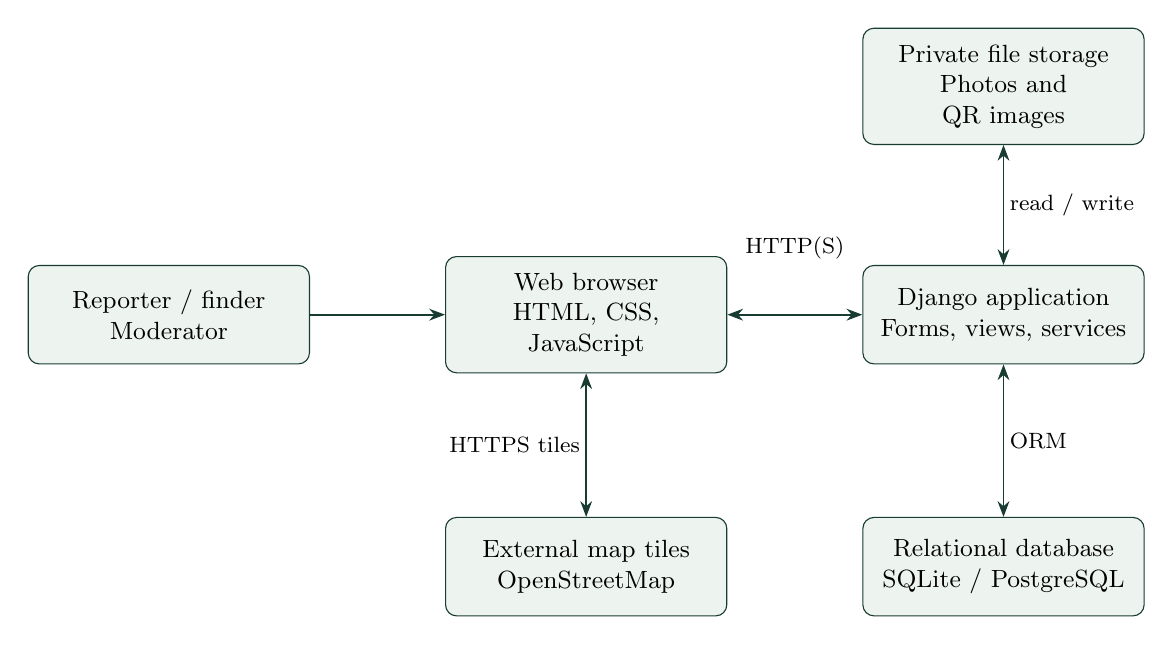
\begin{tikzpicture}[x=1cm,y=1cm,
  ctx/.style={draw=ink,rounded corners=4pt,fill=pale,align=center,
    text width=3.15cm,minimum height=1.25cm,inner sep=6pt,font=\small},
  flow/.style={-{Stealth[length=2mm]},draw=ink,line width=.6pt},
  flowboth/.style={{Stealth[length=2mm]}-{Stealth[length=2mm]},draw=ink,line width=.6pt},
  flowlabel/.style={font=\footnotesize,fill=white,inner sep=2pt,align=center}]
\node[ctx] (people) at (0,1.4) {Reporter / finder\\Moderator};
\node[ctx] (browser) at (5.3,1.4) {Web browser\\HTML, CSS, JavaScript};
\node[ctx] (app) at (10.6,1.4) {Django application\\Forms, views, services};
\node[ctx] (tiles) at (5.3,-1.8) {External map tiles\\OpenStreetMap};
\node[ctx] (db) at (10.6,-1.8) {Relational database\\SQLite / PostgreSQL};
\node[ctx] (files) at (10.6,4.3) {Private file storage\\Photos and QR images};
\draw[flow] (people.east)--(browser.west);
\draw[flowboth] (browser.east)--(app.west);
\node[flowlabel] at (7.95,2.25) {HTTP(S)};
\draw[flowboth] (browser.south)--node[flowlabel,left]{HTTPS tiles}(tiles.north);
\draw[flowboth] (app.south)--node[flowlabel,right]{ORM}(db.north);
\draw[flowboth] (app.north)--node[flowlabel,right]{read / write}(files.south);
\end{tikzpicture}
\caption{System context. The browser requests map tiles directly; Django reads and writes application data and private media.}\label{fig:context}
\end{figure}

\Needspace{14\baselineskip}

\section{Product Functionality}

\begin{itemize}

\item Register an account, sign in by email and password, select session persistence, and sign out.

\item Create a Lost or Found report through Type, Details, Location, Matching and Review steps; save progress on valid submissions.

\item Compare eligible reports using five weighted factors and a minimum private-evidence agreement rule.

\item Review a match, propose or accept a meeting, dismiss or restore an eligible suggestion, and record return.

\item View own dashboard and searchable history, including report status and activity events.

\item Generate a report QR entry route and create, deactivate or reactivate personal item labels.

\item Allow authorized staff to close or remove Open, unreserved reports without exposing private answers.

\end{itemize}

\Needspace{14\baselineskip}

\section{Users and Characteristics}

\begin{longtable}{@{}P{0.29\dimexpr\textwidth-12pt\relax}P{0.71\dimexpr\textwidth-12pt\relax}@{}}

\toprule \textbf{Viewpoint / actor} & \textbf{Needs, characteristics and authority} \\ \midrule\endfirsthead

\toprule \textbf{Viewpoint / actor} & \textbf{Needs, characteristics and authority} \\ \midrule\endhead

\bottomrule\endfoot

Primary: reporter & An everyday user with basic browser skills. May report both Lost and Found items, manage own drafts and labels, and view own reports. \\ \addlinespace[3pt]

Primary: match participant & A reporter involved in a specific pair. Reviews similarities and coordinates return. Can see report contacts only after acceptance. \\ \addlinespace[3pt]

Primary: report QR finder & A person following a report code. Must sign in, then independently complete a Found report using limited prefilled hints. \\ \addlinespace[3pt]

Public: personal-label finder & A person scanning an active item label. No account is needed to see the contact phone intentionally published by its owner. \\ \addlinespace[3pt]

Operational: moderator & Staff account using the management view. Can close/remove eligible reports; has no private-answer inspection function. \\ \addlinespace[3pt]

Operational: system administrator & Deploys the application, manages backups, configuration and account permissions. Database access is outside ordinary browser permissions. \\ \addlinespace[3pt]

Project / assessment & Student team and instructor review scope, traceability and quality; no end-user privileges are implied. \\ \addlinespace[3pt]

\end{longtable}

The application shows public item details while withholding matching answers. Match participants receive contact numbers after the proposed handover is accepted. Moderators can manage reports without viewing private answers.

\Needspace{14\baselineskip}

\section{Operating Environment}

The local project uses Python 3.10 and Django 5.2.17. Development defaults to SQLite; production settings require PostgreSQL, private persistent storage, configured hosts, a secret key and HTTPS. User-facing dates use Asia/Karachi.

\Needspace{12\baselineskip}

\subsection{Observed Live Deployment}

The owner-supplied registration entry point is \url{https://lost-and-found.54.252.227.103.sslip.io/register/}. The public origin is \url{https://lost-and-found.54.252.227.103.sslip.io/}.

\begin{longtable}{@{}P{0.27\dimexpr\textwidth-12pt\relax}P{0.73\dimexpr\textwidth-12pt\relax}@{}}

\toprule \textbf{Deployment detail} & \textbf{Observed value / evidence} \\ \midrule\endfirsthead

\toprule \textbf{Deployment detail} & \textbf{Observed value / evidence} \\ \midrule\endhead

\bottomrule\endfoot

Public identity & Where Is My Stuff? branding and the Report, Review and Arrange workflow appear on the live account pages. \\ \addlinespace[3pt]

DNS destination & The hostname resolved to IPv4 address 54.252.227.103 on 10 October 2026. \\ \addlinespace[3pt]

Transport & Chrome connected with normal certificate validation over TLS 1.3; the certificate subject matched the supplied hostname. \\ \addlinespace[3pt]

Public pages & GET /register/ and GET /login/ returned HTTP 200 and displayed the expected account forms. \\ \addlinespace[3pt]

Access boundary & Anonymous GET requests to /, /reports/, /labels/ and /management/ redirected to /login/ with the requested destination in next. \\ \addlinespace[3pt]

Reported edge server & HTTP Server header reported nginx/1.28.3 (Ubuntu). This identifies the reported web edge, not the complete hosting infrastructure. \\ \addlinespace[3pt]

Code correspondence & The served auth JavaScript was byte-identical to local static/auth.js. Branding, field names and anonymous route behavior also matched the inspected project. \\ \addlinespace[3pt]

Evidence scope & The live database engine, application commit, Python/Django versions, hosting account and authenticated workflows were not exposed by these public observations. \\ \addlinespace[3pt]

\end{longtable}

A modern browser, cookies and JavaScript are required. Camera/QR scanning and printing are optional. No dedicated hardware is required. Minimum server capacity has not been measured; the proposed performance workload is defined in Chapter 4.

\begin{figure}[H]\centering
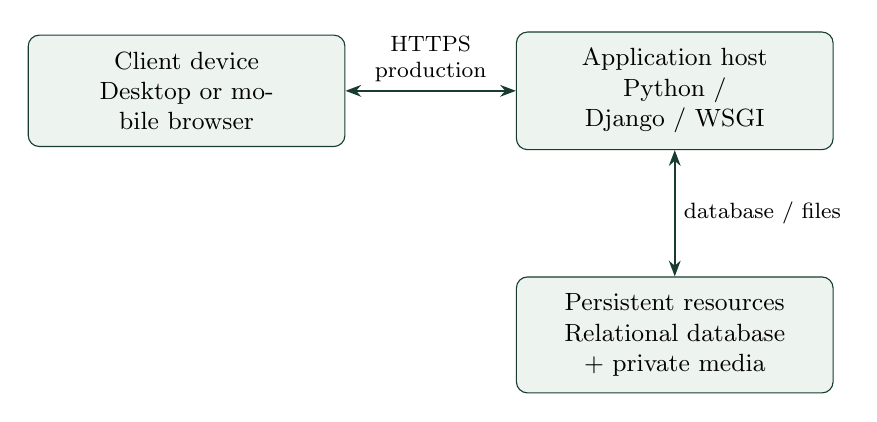
\begin{tikzpicture}[x=1cm,y=1cm,
  env/.style={draw=ink,rounded corners=4pt,fill=pale,align=center,
    text width=3.6cm,minimum height=1.25cm,inner sep=6pt,font=\small},
  flowboth/.style={{Stealth[length=2mm]}-{Stealth[length=2mm]},draw=ink,line width=.6pt},
  flowlabel/.style={font=\footnotesize,fill=white,inner sep=3pt,align=center}]
\node[env] (client) at (0,1.3) {Client device\\Desktop or mobile browser};
\node[env] (host) at (6.2,1.3) {Application host\\Python / Django / WSGI};
\node[env] (persist) at (6.2,-1.8) {Persistent resources\\Relational database + private media};
\draw[flowboth] (client.east)--node[flowlabel,above]{HTTPS\\production}(host.west);
\draw[flowboth] (host.south)--node[flowlabel,right]{database / files}(persist.north);
\end{tikzpicture}
\caption{Deployment environment. Public traffic uses HTTPS; localhost development uses HTTP.}
\end{figure}

\Needspace{14\baselineskip}

\section{Design and Implementation Constraints}

\begin{itemize}

\item DC-01: Use the existing Django 5.2.17 monolith and server-rendered template architecture.

\item DC-02: Keep matching deterministic with the documented weights, minimum score and minimum private agreements; photographs do not contribute to similarity.

\item DC-03: Persist schema changes through Django migrations and preserve unique Lost/Found pairs. PostgreSQL workflows use a transaction advisory lock; the default SQLite configuration uses IMMEDIATE transactions.

\item DC-04: Store uploaded media outside a publicly served directory and authorize each media request.

\item DC-05: Preserve the five-step report workflow and the eight defined categories.

\item DC-06: Use Asia/Karachi for user-facing date/time interpretation. Event dates use DD-MM-YYYY; meetings use DD-MM-YY hh:mm AM/PM.

\item DC-07: Keep readable location text and manual latitude/longitude available independently of map tile loading. No geocoding service is implemented.

\item DC-08: Do not present a match, account or QR scan as proof of ownership or a guaranteed return.

\item DC-09: Production requires environment-supplied secrets, explicit allowed hosts, PostgreSQL and persistent private storage; development defaults are not a production acceptance result.

\end{itemize}

\Needspace{14\baselineskip}

\section{User Documentation}

The interface provides field labels, hints and validation errors. The project README covers setup; a user guide is not included in the current application.

\Needspace{14\baselineskip}

\section{Assumptions and Dependencies}

\begin{itemize}

\item Users supply truthful item descriptions, independently observed locations and reachable contact numbers; the system cannot validate these claims.

\item Users can reach the app and allow session cookies. JavaScript supports dynamic questionnaires and maps; server validation remains authoritative.

\item Django, Pillow, qrcode, dj-database-url, python-dotenv and the PostgreSQL driver are application dependencies. The pinned Django version is 5.2.17; other declared dependency ranges remain those in requirements files.

\item External map tiles may be unavailable; typed location details and valid coordinates remain required and can be supplied manually. Browser geolocation depends on device permission and browser support.

\item Public QR URLs depend on a stable, reachable application hostname. Codes created on localhost are demonstration artifacts.

\item Operators are responsible for secure hosting, storage access and backup policy. Public deployment requires decisions on sensitive identifier collection and retention.

\end{itemize}

\chapter{Specific Requirements}

\Needspace{14\baselineskip}

\section{External Interface Requirements}

\Needspace{12\baselineskip}

\subsection{User Interfaces}

\begin{longtable}{@{}P{0.27\dimexpr\textwidth-12pt\relax}P{0.73\dimexpr\textwidth-12pt\relax}@{}}

\toprule \textbf{Screen / UI ID} & \textbf{Required behavior} \\ \midrule\endfirsthead

\toprule \textbf{Screen / UI ID} & \textbf{Required behavior} \\ \midrule\endhead

\bottomrule\endfoot

UI-01: account screens & Register with full name, unique email and validated password; sign in with email/password and remember-me; display actionable validation errors. \\ \addlinespace[3pt]

UI-02: report wizard & Show five ordered stages: Type, Details, Location, Matching, Review. Save a valid step on Save and next. Back links permit changes. Do not claim keystroke autosave. \\ \addlinespace[3pt]

UI-03: location & Provide a readable place, location description, map pin controls, optional device location, and manual latitude/longitude fields. \\ \addlinespace[3pt]

UI-04: dashboard / history & Show owner-specific summaries, saved drafts and active matches. Show all non-Removed owned reports through searchable, filtered, paginated history. \\ \addlinespace[3pt]

UI-05: review / match & Review public report fields and photo; keep phone/private answers on their earlier steps. Match page shows paired public descriptions and factor scores, meeting controls and conditional contacts. \\ \addlinespace[3pt]

UI-06: QR labels & Show item name, chosen phone, expiry and activation status; allow owner image download and state controls. Public scan distinguishes active from inactive. \\ \addlinespace[3pt]

UI-07: moderation & Expose a staff-only report list and eligible close/remove controls without private answers. \\ \addlinespace[3pt]

UI-08: responsive target & Proposed: at 360 CSS pixels width, core form controls and primary actions shall be usable without horizontal page scrolling. Verify separately from desktop observations. \\ \addlinespace[3pt]

\end{longtable}

Common interface conventions are labeled fields, consistent navigation, back/cancel actions, visible report IDs and status, and inline form errors. Success notices follow a saved step or action. Appendix C contains localhost screenshots using synthetic data. Appendix D contains live registration/login screenshots. The figures identify their environment and do not constitute a complete usability or accessibility audit.

Figures 3.1-3.2 show the dashboard, report flow and match-review design. Current implementation screens are shown in Appendix C.

\begin{figure}[H]\centering\includegraphics[width=\textwidth,height=.48\textheight,keepaspectratio]{wireframe-live-reference.png}\caption{Dashboard and match-review wireframes; the adjacent QR and live-login panels are design references.}\end{figure}

\begin{figure}[H]\centering\includegraphics[width=\textwidth,height=.24\textheight,keepaspectratio]{wireframe-report-flow.png}\caption{Five-step report flow: Type, Details, Location, Matching and Review.}\end{figure}

\Needspace{12\baselineskip}

\subsection{Match Review and Handover Interaction}

The match view shows paired public summaries and score factors. It withholds contacts until the other participant accepts; private answers remain hidden. A match score does not verify ownership.

\Needspace{12\baselineskip}

\subsection{Hardware Interfaces}

The application has no direct proprietary hardware interface. Browser file upload accepts an optional image from disk or a camera source supported by the device. Browser geolocation may provide latitude and longitude after user permission. QR codes are PNG images that can be printed and scanned by standard camera software; printing and scanning remain device/browser functions.

\Needspace{12\baselineskip}

\subsection{Software Interfaces}

\begin{longtable}{@{}P{0.29\dimexpr\textwidth-12pt\relax}P{0.71\dimexpr\textwidth-12pt\relax}@{}}

\toprule \textbf{Component} & \textbf{Interface and exchanged information} \\ \midrule\endfirsthead

\toprule \textbf{Component} & \textbf{Interface and exchanged information} \\ \midrule\endhead

\bottomrule\endfoot

Django and operating system & Python processes read static resources and configuration, use the system clock and write media through filesystem APIs. A writable private media directory is required. \\ \addlinespace[3pt]

Relational database & Django ORM reads/writes User, Report, Draft, Match, Event and QRLabel records. SQLite is the development default; PostgreSQL is required by the production settings. \\ \addlinespace[3pt]

Pillow / QR generation & Pillow decodes and normalizes image uploads. The qrcode library encodes report-entry or label URLs as PNG images. \\ \addlinespace[3pt]

Leaflet / map tiles & Locally served Leaflet displays externally fetched map tiles. Coordinates are form data; place text is not sent to a geocoding API. \\ \addlinespace[3pt]

Browser sessions & Django session cookie associates requests with an authenticated user. CSRF tokens protect submitted POST forms. \\ \addlinespace[3pt]

\end{longtable}

\Needspace{12\baselineskip}

\subsection{Communications Interfaces}

Browser requests use HTTP on localhost. The owner-supplied public deployment uses HTTPS, with TLS 1.3 observed on its account pages. Forms use ordinary encoded POST data and multipart upload for images. Views return HTML or protected PNG/JPEG streams; no email, SMS or chat delivery interface is implemented. The browser fetches HTTPS map tiles from tile.openstreetmap.de and retains OpenStreetMap attribution.

Production settings enable secure session/CSRF cookies, HTTPS redirection, explicit hosts and response protections. Uploaded photos and owner-only label images use private, no-store responses. Public personal-label responses also use no-referrer. Only the token digest is stored in the label database field; the downloadable QR image necessarily encodes the bearer URL and must remain protected.

\Needspace{14\baselineskip}

\section{Functional Requirements}

\Needspace{12\baselineskip}

\subsection{User Requirements and System Allocation}

\begin{longtable}{@{}P{0.12\dimexpr\textwidth-24pt\relax}P{0.38\dimexpr\textwidth-24pt\relax}P{0.5\dimexpr\textwidth-24pt\relax}@{}}

\toprule \textbf{ID} & \textbf{User need} & \textbf{Allocated requirements / use case / scenario} \\ \midrule\endfirsthead

\toprule \textbf{ID} & \textbf{User need} & \textbf{Allocated requirements / use case / scenario} \\ \midrule\endhead

\bottomrule\endfoot

UR-01 & Access my account securely. & FR-ACC-01 to 06 / UC-01 / AT-01 \\ \addlinespace[3pt]

UR-02 & Publish a useful Lost or Found report. & FR-REP-01 to 04, 09 to 13; FR-VAL; FR-PHO / UC-02 / AT-02,03 \\ \addlinespace[3pt]

UR-03 & Save and resume unfinished work. & FR-REP-05 to 08,12 / UC-03 / AT-02 \\ \addlinespace[3pt]

UR-04 & See plausible item matches with understandable scores. & FR-MAT-01 to 08 / UC-04 / AT-04 \\ \addlinespace[3pt]

UR-05 & Agree on a meeting and control contact disclosure. & FR-HND-01 to 06,08,09 / UC-05 / AT-05 \\ \addlinespace[3pt]

UR-06 & Record an item as returned after the meeting time. & FR-HND-07; FR-HIS-05 / UC-06 / AT-05 \\ \addlinespace[3pt]

UR-07 & Find my reports, statuses and activity. & FR-HIS-01 to 06 / UC-07 / AT-06 \\ \addlinespace[3pt]

UR-08 & Help a finder start a report using my report QR. & FR-QR-01 to 04,10 / UC-08 / AT-07 \\ \addlinespace[3pt]

UR-09 & Create and control a printable contact label. & FR-QR-05 to 09,11 / UC-09 / AT-07 \\ \addlinespace[3pt]

UR-10 & Moderate eligible reports without viewing private answers. & FR-MOD-01 to 05 / UC-10 / AT-06 \\ \addlinespace[3pt]

\end{longtable}

The following requirements retain the original IDs and priorities. Acceptance statements define the expected observable outcome. The traceability matrix links each family to code locations and planned scenario coverage; the limited observations actually performed are recorded separately.

\Needspace{12\baselineskip}

\subsection{Accounts and Authorization}

\Needspace{6\baselineskip}\noindent\begin{minipage}{\linewidth}\textbf{FR-ACC-01}\hfill\textit{High}\par\nopagebreak

The system shall let a visitor register with a name, unique email address, and a password that satisfies configured password validators.

{\color{muted}\textbf{Acceptance:} Valid unused credentials create one account and sign the user in; a duplicate email or password failing validators creates none and produces an error.\par}\end{minipage}\par\vspace{5pt}

\Needspace{6\baselineskip}\noindent\begin{minipage}{\linewidth}\textbf{FR-ACC-02}\hfill\textit{High}\par\nopagebreak

The system shall authenticate a registered user using email and password and offer a remember-me session choice.

{\color{muted}\textbf{Acceptance:} Valid credentials establish a session; invalid credentials establish none. The remember-me choice controls session expiry.\par}\end{minipage}\par\vspace{5pt}

\Needspace{6\baselineskip}\noindent\begin{minipage}{\linewidth}\textbf{FR-ACC-03}\hfill\textit{High}\par\nopagebreak

The system shall allow an authenticated user to sign out.

{\color{muted}\textbf{Acceptance:} After sign-out, a protected request requires authentication.\par}\end{minipage}\par\vspace{5pt}

\Needspace{6\baselineskip}\noindent\begin{minipage}{\linewidth}\textbf{FR-ACC-04}\hfill\textit{High}\par\nopagebreak

The system shall require authentication for protected reports, drafts, matches, history, dashboard, and label management.

{\color{muted}\textbf{Acceptance:} A signed-out request discloses no protected data and asks the visitor to authenticate.\par}\end{minipage}\par\vspace{5pt}

\Needspace{6\baselineskip}\noindent\begin{minipage}{\linewidth}\textbf{FR-ACC-05}\hfill\textit{High}\par\nopagebreak

The system shall restrict report/draft actions to the owner, match actions to participants, and moderation actions to staff.

{\color{muted}\textbf{Acceptance:} An actor lacking the required relationship/role is denied and the record remains unchanged.\par}\end{minipage}\par\vspace{5pt}

\Needspace{6\baselineskip}\noindent\begin{minipage}{\linewidth}\textbf{FR-ACC-06}\hfill\textit{High}\par\nopagebreak

The system shall protect submitted state-changing POST forms against cross-site request forgery.

{\color{muted}\textbf{Acceptance:} A POST with a missing or invalid token is rejected without applying the submitted action. GET routes that create or update drafts are a documented limitation in Chapter 5.\par}\end{minipage}\par\vspace{5pt}

\Needspace{12\baselineskip}

\subsection{Reports and Drafts}

\Needspace{6\baselineskip}\noindent\begin{minipage}{\linewidth}\textbf{FR-REP-01}\hfill\textit{High}\par\nopagebreak

The system shall let an authenticated user create a Lost or Found report.

{\color{muted}\textbf{Acceptance:} User can select either report kind; all later report behavior preserves that selection.\par}\end{minipage}\par\vspace{5pt}

\Needspace{6\baselineskip}\noindent\begin{minipage}{\linewidth}\textbf{FR-REP-02}\hfill\textit{High}\par\nopagebreak

A report shall record category, title, event date, public description, contact phone, readable place name, required location description, latitude, and longitude. All listed fields are required to publish.

{\color{muted}\textbf{Acceptance:} Missing or invalid data in any required field, including location description or either coordinate, prevents publication; valid values are saved with the report.\par}\end{minipage}\par\vspace{5pt}

\Needspace{6\baselineskip}\noindent\begin{minipage}{\linewidth}\textbf{FR-REP-03}\hfill\textit{Medium}\par\nopagebreak

A report may include one photograph.

{\color{muted}\textbf{Acceptance:} The photograph may be omitted; when supplied it is associated with the report and protected under FR-PHO-04, NFR-SEC-08, and SEC-05.\par}\end{minipage}\par\vspace{5pt}

\Needspace{6\baselineskip}\noindent\begin{minipage}{\linewidth}\textbf{FR-REP-04}\hfill\textit{High}\par\nopagebreak

The system shall ask category-appropriate private questions and store answers with the report.

{\color{muted}\textbf{Acceptance:} Each supported category presents applicable questions; required and conditional answers are validated before publication.\par}\end{minipage}\par\vspace{5pt}

\Needspace{6\baselineskip}\noindent\begin{minipage}{\linewidth}\textbf{FR-REP-05}\hfill\textit{High}\par\nopagebreak

The system shall save draft progress whenever a valid wizard step is submitted.

{\color{muted}\textbf{Acceptance:} After submitting a valid step and leaving the flow, the draft contains that step's values.\par}\end{minipage}\par\vspace{5pt}

\Needspace{6\baselineskip}\noindent\begin{minipage}{\linewidth}\textbf{FR-REP-06}\hfill\textit{High}\par\nopagebreak

The system shall let an owner resume saved draft data. Public fields and ordinary private choices shall be repopulated. Identifier inputs shall stay masked and shall not reprint stored values.

{\color{muted}\textbf{Acceptance:} Saved fields persist after navigation; password-style identifier fields display blank and may require re-entry if the Matching step is resubmitted.\par}\end{minipage}\par\vspace{5pt}

\Needspace{6\baselineskip}\noindent\begin{minipage}{\linewidth}\textbf{FR-REP-07}\hfill\textit{Medium}\par\nopagebreak

The system shall require explicit confirmation before discarding an existing draft to start another.

{\color{muted}\textbf{Acceptance:} Cancel preserves the draft; confirmation discards it and permits a new draft.\par}\end{minipage}\par\vspace{5pt}

\Needspace{6\baselineskip}\noindent\begin{minipage}{\linewidth}\textbf{FR-REP-08}\hfill\textit{High}\par\nopagebreak

A user shall not be able to read, edit, or delete another user's draft.

{\color{muted}\textbf{Acceptance:} A different account receives denial/not-found and cannot alter or infer draft contents.\par}\end{minipage}\par\vspace{5pt}

\Needspace{6\baselineskip}\noindent\begin{minipage}{\linewidth}\textbf{FR-REP-09}\hfill\textit{High}\par\nopagebreak

The review step shall show the owner a summary of report type/category, title, event date, public description, location, and any photo. Private answers and contact phone shall remain on their earlier wizard steps and shall not be included in the review summary.

{\color{muted}\textbf{Acceptance:} The review summary shows the listed values and no private-answer or phone values; the owner can return to earlier steps to inspect or change them.\par}\end{minipage}\par\vspace{5pt}

\Needspace{6\baselineskip}\noindent\begin{minipage}{\linewidth}\textbf{FR-REP-10}\hfill\textit{Medium}\par\nopagebreak

The system shall let an owner edit an open report that is not reserved for handover.

{\color{muted}\textbf{Acceptance:} Eligible report can be edited; closed or reserved report cannot be changed.\par}\end{minipage}\par\vspace{5pt}

\Needspace{6\baselineskip}\noindent\begin{minipage}{\linewidth}\textbf{FR-REP-11}\hfill\textit{High}\par\nopagebreak

The system shall run matching after a report is published.

{\color{muted}\textbf{Acceptance:} A newly published report is evaluated against eligible opposite-kind reports and qualifying matches are available to participants.\par}\end{minipage}\par\vspace{5pt}

\Needspace{6\baselineskip}\noindent\begin{minipage}{\linewidth}\textbf{FR-REP-12}\hfill\textit{Medium}\par\nopagebreak

When a draft's category is changed, the system shall clear private answers that belong to the previous category.

{\color{muted}\textbf{Acceptance:} After a category change, old-category answer keys appear in neither the revised draft nor review.\par}\end{minipage}\par\vspace{5pt}

\Needspace{6\baselineskip}\noindent\begin{minipage}{\linewidth}\textbf{FR-REP-13}\hfill\textit{Medium}\par\nopagebreak

Each report shall have a display identifier built from its kind and database ID (LFD-... for Lost, FND-... for Found) and a separate UUID used in report QR URLs. The database ID shall not appear in QR URLs.

{\color{muted}\textbf{Acceptance:} A Lost report shows an LFD- identifier and a Found report an FND- identifier; its report QR URL contains the UUID.\par}\end{minipage}\par\vspace{5pt}

\Needspace{12\baselineskip}

\subsection{Input Validation}

\Needspace{6\baselineskip}\noindent\begin{minipage}{\linewidth}\textbf{FR-VAL-01}\hfill\textit{High}\par\nopagebreak

The system shall reject title, place, location detail, or description text that matches configured private-identifier patterns.

{\color{muted}\textbf{Acceptance:} Identifiers within configured detection rules are rejected; submitted text is not silently rewritten.\par}\end{minipage}\par\vspace{5pt}

\Needspace{6\baselineskip}\noindent\begin{minipage}{\linewidth}\textbf{FR-VAL-02}\hfill\textit{High}\par\nopagebreak

The system shall reject public text containing configured invisible or control characters.

{\color{muted}\textbf{Acceptance:} Submitted characters covered by the configured rule cause a field error and no publication.\par}\end{minipage}\par\vspace{5pt}

\Needspace{6\baselineskip}\noindent\begin{minipage}{\linewidth}\textbf{FR-VAL-03}\hfill\textit{High}\par\nopagebreak

When public text is rejected, the system shall explain the validation failure and preserve the submitted value for correction.

{\color{muted}\textbf{Acceptance:} The user sees an actionable error and can edit the unchanged submitted value.\par}\end{minipage}\par\vspace{5pt}

\Needspace{6\baselineskip}\noindent\begin{minipage}{\linewidth}\textbf{FR-VAL-04}\hfill\textit{Medium}\par\nopagebreak

The system shall require the reported event date not to be in the future and not before 1 January 2000.

{\color{muted}\textbf{Acceptance:} A future date or date before 1 January 2000 is rejected; today or an allowed past date is accepted.\par}\end{minipage}\par\vspace{5pt}

\Needspace{6\baselineskip}\noindent\begin{minipage}{\linewidth}\textbf{FR-VAL-05}\hfill\textit{Medium}\par\nopagebreak

The system shall require latitude and longitude to fall within valid geographic ranges (latitude -90 to 90, longitude -180 to 180). The system does not restrict points to a service-area boundary.

{\color{muted}\textbf{Acceptance:} A point inside valid ranges is accepted; a point outside them is refused.\par}\end{minipage}\par\vspace{5pt}

\Needspace{6\baselineskip}\noindent\begin{minipage}{\linewidth}\textbf{FR-VAL-06}\hfill\textit{High}\par\nopagebreak

The system shall render user-entered text as data rather than executable markup or script.

{\color{muted}\textbf{Acceptance:} Script/markup test strings render inertly in report, match, history, and staff views.\par}\end{minipage}\par\vspace{5pt}

\Needspace{12\baselineskip}

\subsection{Photographs}

\Needspace{6\baselineskip}\noindent\begin{minipage}{\linewidth}\textbf{FR-PHO-01}\hfill\textit{Medium}\par\nopagebreak

The system shall accept a photo only if its type, size, and pixel dimensions are within configured limits.

{\color{muted}\textbf{Acceptance:} A valid in-limit photo is accepted; each out-of-limit sample is refused without losing other draft data.\par}\end{minipage}\par\vspace{5pt}

\Needspace{6\baselineskip}\noindent\begin{minipage}{\linewidth}\textbf{FR-PHO-02}\hfill\textit{Medium}\par\nopagebreak

The system shall decode each uploaded image and reject damaged or non-image files.

{\color{muted}\textbf{Acceptance:} Renamed non-image and corrupted image files are refused.\par}\end{minipage}\par\vspace{5pt}

\Needspace{6\baselineskip}\noindent\begin{minipage}{\linewidth}\textbf{FR-PHO-03}\hfill\textit{Medium}\par\nopagebreak

The system shall normalize accepted photos to JPEG, resize the longest edge to at most 1,800 pixels, and discard source metadata before storage.

{\color{muted}\textbf{Acceptance:} Retrieved image is JPEG, is no larger than 1,800 pixels on its longest edge, and has no carried source metadata.\par}\end{minipage}\par\vspace{5pt}

\Needspace{6\baselineskip}\noindent\begin{minipage}{\linewidth}\textbf{FR-PHO-04}\hfill\textit{High}\par\nopagebreak

The system shall serve report photographs only to the report owner and an owner of the opposite report in a match involving that report.

{\color{muted}\textbf{Acceptance:} Authorized requests return the image; unrelated/anonymous requests return no image bytes.\par}\end{minipage}\par\vspace{5pt}

Upload limits: JPEG, PNG or WebP; at most 5 MiB; at most 6,000 pixels per side and 24,000,000 pixels total. Accepted images are decoded, orientation-corrected, resized without cropping, flattened on white when transparent, converted to RGB and stored as JPEG with a maximum 1,800-pixel edge. No visual recognition is performed.

\Needspace{12\baselineskip}

\subsection{Matching}

\Needspace{6\baselineskip}\noindent\begin{minipage}{\linewidth}\textbf{FR-MAT-01}\hfill\textit{High}\par\nopagebreak

The system shall compare a published report with opposite-kind, same-category Open reports owned by other users, excluding reserved candidates. Scoring shall reject same-owner, wrong-kind, closed or different-category pairs.

{\color{muted}\textbf{Acceptance:} Publishing creates no new suggestion against a reserved candidate or a pair violating a scoring condition.\par}\end{minipage}\par\vspace{5pt}

\Needspace{6\baselineskip}\noindent\begin{minipage}{\linewidth}\textbf{FR-MAT-02}\hfill\textit{High}\par\nopagebreak

The system shall require at least two meaningful private-answer agreements for a possible match.

{\color{muted}\textbf{Acceptance:} Fewer than two agreements produces no match even when other factors score maximally.\par}\end{minipage}\par\vspace{5pt}

\Needspace{6\baselineskip}\noindent\begin{minipage}{\linewidth}\textbf{FR-MAT-03}\hfill\textit{High}\par\nopagebreak

The system shall score an eligible pair from 0 to 100 using category (20), location (20), date (15), description (15), and private answers (30).

{\color{muted}\textbf{Acceptance:} Controlled factor fixtures produce the documented weighted sum, always between 0 and 100.\par}\end{minipage}\par\vspace{5pt}

\Needspace{6\baselineskip}\noindent\begin{minipage}{\linewidth}\textbf{FR-MAT-04}\hfill\textit{High}\par\nopagebreak

The system shall create a possible match only when its score is at least 70.

{\color{muted}\textbf{Acceptance:} Score 69 creates none; score 70 with at least two private agreements creates one.\par}\end{minipage}\par\vspace{5pt}

\Needspace{6\baselineskip}\noindent\begin{minipage}{\linewidth}\textbf{FR-MAT-05}\hfill\textit{High}\par\nopagebreak

The system shall store each match's score and factor scores.

{\color{muted}\textbf{Acceptance:} Match detail displays the correct factor totals for the test pair.\par}\end{minipage}\par\vspace{5pt}

\Needspace{6\baselineskip}\noindent\begin{minipage}{\linewidth}\textbf{FR-MAT-06}\hfill\textit{High}\par\nopagebreak

The system shall create at most one match for a given Lost/Found report pair.

{\color{muted}\textbf{Acceptance:} Repeated publication/recalculation of the same pair does not create duplicate matches.\par}\end{minipage}\par\vspace{5pt}

\Needspace{6\baselineskip}\noindent\begin{minipage}{\linewidth}\textbf{FR-MAT-07}\hfill\textit{High}\par\nopagebreak

The match page shall show factor scores without exposing the other party's private-answer values.

{\color{muted}\textbf{Acceptance:} Participants can see factor agreement; raw private responses remain absent.\par}\end{minipage}\par\vspace{5pt}

\Needspace{6\baselineskip}\noindent\begin{minipage}{\linewidth}\textbf{FR-MAT-08}\hfill\textit{High}\par\nopagebreak

The match page shall state that a match is not proof of ownership.

{\color{muted}\textbf{Acceptance:} The notice is visible on each match detail page.\par}\end{minipage}\par\vspace{5pt}

\Needspace{12\baselineskip}

\subsection{Handover and Return}

\Needspace{6\baselineskip}\noindent\begin{minipage}{\linewidth}\textbf{FR-HND-01}\hfill\textit{High}\par\nopagebreak

A participant shall be able to propose a meeting place and future time for a possible match.

{\color{muted}\textbf{Acceptance:} A non-empty place and future time create a proposal; invalid time or reserved reports prevent the proposal.\par}\end{minipage}\par\vspace{5pt}

\Needspace{6\baselineskip}\noindent\begin{minipage}{\linewidth}\textbf{FR-HND-02}\hfill\textit{High}\par\nopagebreak

The other participant shall be able to accept the pending proposal. Either participant may dismiss a possible match or pending proposal.

{\color{muted}\textbf{Acceptance:} The non-proposer's acceptance schedules the handover. Dismissal sets the match to Rejected and releases any reservation for a pending proposal.\par}\end{minipage}\par\vspace{5pt}

\Needspace{6\baselineskip}\noindent\begin{minipage}{\linewidth}\textbf{FR-HND-03}\hfill\textit{High}\par\nopagebreak

The proposer shall not accept their own proposal as the second participant.

{\color{muted}\textbf{Acceptance:} Proposer acceptance is refused and state remains pending.\par}\end{minipage}\par\vspace{5pt}

\Needspace{6\baselineskip}\noindent\begin{minipage}{\linewidth}\textbf{FR-HND-04}\hfill\textit{Low}\par\nopagebreak

Only the participant who dismissed a suggestion shall be able to restore it, and only if neither report is reserved and the pair still meets current match rules.

{\color{muted}\textbf{Acceptance:} The dismissing participant restores an eligible pair; the other participant cannot restore it; stale, ineligible, or conflicting pair remains rejected.\par}\end{minipage}\par\vspace{5pt}

\Needspace{6\baselineskip}\noindent\begin{minipage}{\linewidth}\textbf{FR-HND-05}\hfill\textit{High}\par\nopagebreak

The system shall show both saved report contact numbers to match participants after the other participant accepts the handover.

{\color{muted}\textbf{Acceptance:} Both participants see the numbers in Handover Scheduled and Returned states.\par}\end{minipage}\par\vspace{5pt}

\Needspace{6\baselineskip}\noindent\begin{minipage}{\linewidth}\textbf{FR-HND-06}\hfill\textit{High}\par\nopagebreak

The system shall withhold both saved report contact numbers while a match is Possible Match or Handover Proposed.

{\color{muted}\textbf{Acceptance:} Neither participant sees the numbers before the other participant accepts.\par}\end{minipage}\par\vspace{5pt}

\Needspace{6\baselineskip}\noindent\begin{minipage}{\linewidth}\textbf{FR-HND-07}\hfill\textit{High}\par\nopagebreak

A participant shall be able to record return only at or after the scheduled meeting time. On return, both reports become Returned, reservations are cleared, and competing possible matches involving either report are dismissed.

{\color{muted}\textbf{Acceptance:} Early return is refused; at or after meeting time it succeeds and updates both reports and competing matches.\par}\end{minipage}\par\vspace{5pt}

\Needspace{6\baselineskip}\noindent\begin{minipage}{\linewidth}\textbf{FR-HND-08}\hfill\textit{High}\par\nopagebreak

While a handover is proposed or scheduled, the system shall reserve its reports against editing, moderation, or a second active handover.

{\color{muted}\textbf{Acceptance:} Competing proposals allow at most one active reservation; edit/moderation attempts fail while reserved.\par}\end{minipage}\par\vspace{5pt}

\Needspace{6\baselineskip}\noindent\begin{minipage}{\linewidth}\textbf{FR-HND-09}\hfill\textit{High}\par\nopagebreak

Only a participant of a match shall be able to view or change its state.

{\color{muted}\textbf{Acceptance:} Nonparticipant read and action requests are denied without disclosure or state change.\par}\end{minipage}\par\vspace{5pt}

An existing scheduled handover has no cancel, reschedule or timeout action in the baseline. A return is recorded by either participant, with no second return confirmation. These limitations are reflected in the state model rather than implied as missing transitions.

\Needspace{12\baselineskip}

\subsection{Dashboard and History}

\Needspace{6\baselineskip}\noindent\begin{minipage}{\linewidth}\textbf{FR-HIS-01}\hfill\textit{High}\par\nopagebreak

The dashboard shall show the signed-in user's summaries, drafts and active matches. It shall show at most three Open reports and ten returned reports, with full report access through history.

{\color{muted}\textbf{Acceptance:} The dashboard shows only owned reports, prioritizes handover actions and hides possible matches whose reports are reserved. Users with no visible reports enter the report/draft flow.\par}\end{minipage}\par\vspace{5pt}

\Needspace{6\baselineskip}\noindent\begin{minipage}{\linewidth}\textbf{FR-HIS-02}\hfill\textit{Medium}\par\nopagebreak

The history page shall list the user's non-Removed reports and support search by title/location and filters for kind and status.

{\color{muted}\textbf{Acceptance:} Combined query and filters return only matching records owned by that user.\par}\end{minipage}\par\vspace{5pt}

\Needspace{6\baselineskip}\noindent\begin{minipage}{\linewidth}\textbf{FR-HIS-03}\hfill\textit{Low}\par\nopagebreak

The history page shall divide long lists into pages of ten reports.

{\color{muted}\textbf{Acceptance:} More than ten records are accessible across pages.\par}\end{minipage}\par\vspace{5pt}

\Needspace{6\baselineskip}\noindent\begin{minipage}{\linewidth}\textbf{FR-HIS-04}\hfill\textit{High}\par\nopagebreak

The user shall see only their own reports in dashboard and history.

{\color{muted}\textbf{Acceptance:} Two-account fixture demonstrates strict owner separation.\par}\end{minipage}\par\vspace{5pt}

\Needspace{6\baselineskip}\noindent\begin{minipage}{\linewidth}\textbf{FR-HIS-05}\hfill\textit{Medium}\par\nopagebreak

The system shall persist actor and timestamp for report creation/edit, match state transitions, moderation and return events.

{\color{muted}\textbf{Acceptance:} Each action writes an Event row for every affected report. The report activity view displays event text and time; actor identity remains available in the stored record.\par}\end{minipage}\par\vspace{5pt}

\Needspace{6\baselineskip}\noindent\begin{minipage}{\linewidth}\textbf{FR-HIS-06}\hfill\textit{Medium}\par\nopagebreak

The system shall reject history search strings that contain configured invisible or control characters.

{\color{muted}\textbf{Acceptance:} Such a query returns a client error and exposes no additional report data.\par}\end{minipage}\par\vspace{5pt}

\Needspace{12\baselineskip}

\subsection{Report QR and Personal Labels}

\Needspace{6\baselineskip}\noindent\begin{minipage}{\linewidth}\textbf{FR-QR-01}\hfill\textit{Medium}\par\nopagebreak

The system shall generate a QR code containing the UUID URL of a report. The standard report interface offers this code for Lost reports.

{\color{muted}\textbf{Acceptance:} The UUID URL opens the report-entry flow. The endpoint does not enforce Lost kind; see GAP-04.\par}\end{minipage}\par\vspace{5pt}

\Needspace{6\baselineskip}\noindent\begin{minipage}{\linewidth}\textbf{FR-QR-02}\hfill\textit{Medium}\par\nopagebreak

A signed-in finder opening an eligible report QR shall create or reuse their newest new-report draft and seed kind Found, category, title, coarse place and today's date. The flow shall clear description, detailed location, contact, answers and coordinates before completion.

{\color{muted}\textbf{Acceptance:} No report is automatically published. The finder must supply their own remaining fields. This flow can overwrite an existing new-report draft; see Chapter 5.\par}\end{minipage}\par\vspace{5pt}

\Needspace{6\baselineskip}\noindent\begin{minipage}{\linewidth}\textbf{FR-QR-03}\hfill\textit{High}\par\nopagebreak

The report QR shall not reveal private answers or the owner's phone number.

{\color{muted}\textbf{Acceptance:} QR URL and seeded draft contain neither private answers nor contact number.\par}\end{minipage}\par\vspace{5pt}

\Needspace{6\baselineskip}\noindent\begin{minipage}{\linewidth}\textbf{FR-QR-04}\hfill\textit{Medium}\par\nopagebreak

A signed-out finder opening the report QR shall be asked to sign in before report hints are copied into a draft.

{\color{muted}\textbf{Acceptance:} Before sign-in no seeded draft is created; after sign-in eligible hints may be copied.\par}\end{minipage}\par\vspace{5pt}

\Needspace{6\baselineskip}\noindent\begin{minipage}{\linewidth}\textbf{FR-QR-05}\hfill\textit{Medium}\par\nopagebreak

A user shall be able to create a personal label with an item name and phone number. The label's expiry is fixed at six months after creation.

{\color{muted}\textbf{Acceptance:} A created label expires six months after creation; the user cannot choose another expiry.\par}\end{minipage}\par\vspace{5pt}

\Needspace{6\baselineskip}\noindent\begin{minipage}{\linewidth}\textbf{FR-QR-06}\hfill\textit{High}\par\nopagebreak

The QRLabel database row shall store a SHA-256 digest of the personal-label bearer token in token\_hash and no separate raw-token field.

{\color{muted}\textbf{Acceptance:} The row contains the digest and resolves a presented token. The stored QR image still encodes the token URL and is available only through owner-authorized image access.\par}\end{minipage}\par\vspace{5pt}

\Needspace{6\baselineskip}\noindent\begin{minipage}{\linewidth}\textbf{FR-QR-07}\hfill\textit{Medium}\par\nopagebreak

Scanning an active personal label shall show the phone number its owner chose to publish.

{\color{muted}\textbf{Acceptance:} An active, unexpired, unrevoked token displays its associated number.\par}\end{minipage}\par\vspace{5pt}

\Needspace{6\baselineskip}\noindent\begin{minipage}{\linewidth}\textbf{FR-QR-08}\hfill\textit{High}\par\nopagebreak

Scanning an expired, revoked, or deactivated label shall not show a phone number.

{\color{muted}\textbf{Acceptance:} All inactive conditions suppress the number.\par}\end{minipage}\par\vspace{5pt}

\Needspace{6\baselineskip}\noindent\begin{minipage}{\linewidth}\textbf{FR-QR-09}\hfill\textit{Medium}\par\nopagebreak

An owner shall be able to deactivate or reactivate a personal label. Reactivation shall set expiry to six calendar months from the reactivation time.

{\color{muted}\textbf{Acceptance:} Deactivation hides the number. Reactivation preserves the printed token and enables it until the newly calculated expiry; month-end days are clamped to the target month.\par}\end{minipage}\par\vspace{5pt}

\Needspace{6\baselineskip}\noindent\begin{minipage}{\linewidth}\textbf{FR-QR-10}\hfill\textit{Medium}\par\nopagebreak

The system shall refuse self-use of a report QR and show a notice when the source report is closed or reserved.

{\color{muted}\textbf{Acceptance:} The owner is returned to their report; a closed/reserved source seeds no Found draft and shows a notice.\par}\end{minipage}\par\vspace{5pt}

\Needspace{6\baselineskip}\noindent\begin{minipage}{\linewidth}\textbf{FR-QR-11}\hfill\textit{Medium}\par\nopagebreak

The label owner shall be able to view and download the label's QR image. Other accounts shall not access it.

{\color{muted}\textbf{Acceptance:} Owner receives the image; a non-owner receives denial or not-found.\par}\end{minipage}\par\vspace{5pt}

The report detail UI presents report QR codes for Open Lost reports. The underlying UUID routes do not enforce kind=Lost and the QR PNG endpoint is public to anyone with the UUID. A public UUID image contains a URL, not report contacts or private answers. The personal-label workflow is separate: an active bearer URL deliberately exposes the chosen phone without authentication.

\Needspace{12\baselineskip}

\subsection{Moderation}

\Needspace{6\baselineskip}\noindent\begin{minipage}{\linewidth}\textbf{FR-MOD-01}\hfill\textit{Medium}\par\nopagebreak

The system shall provide staff with a report-management list of non-Removed reports.

{\color{muted}\textbf{Acceptance:} Authorized staff can access the list.\par}\end{minipage}\par\vspace{5pt}

\Needspace{6\baselineskip}\noindent\begin{minipage}{\linewidth}\textbf{FR-MOD-02}\hfill\textit{Medium}\par\nopagebreak

A staff user shall be able to close or remove an open report that is not reserved. The action shall dismiss its possible matches.

{\color{muted}\textbf{Acceptance:} Eligible report changes state and possible matches become Rejected; closed, removed, or reserved report action is refused. A Removed report leaves ordinary history and management lists.\par}\end{minipage}\par\vspace{5pt}

\Needspace{6\baselineskip}\noindent\begin{minipage}{\linewidth}\textbf{FR-MOD-03}\hfill\textit{High}\par\nopagebreak

The management list shall not show private answers.

{\color{muted}\textbf{Acceptance:} Private answer values do not appear in management output.\par}\end{minipage}\par\vspace{5pt}

\Needspace{6\baselineskip}\noindent\begin{minipage}{\linewidth}\textbf{FR-MOD-04}\hfill\textit{Medium}\par\nopagebreak

Each moderation action shall record the acting staff user and event time.

{\color{muted}\textbf{Acceptance:} Resulting event identifies the actor and timestamp.\par}\end{minipage}\par\vspace{5pt}

\Needspace{6\baselineskip}\noindent\begin{minipage}{\linewidth}\textbf{FR-MOD-05}\hfill\textit{High}\par\nopagebreak

A non-staff user shall be denied access to management functions.

{\color{muted}\textbf{Acceptance:} Non-staff request is denied without exposing the management list.\par}\end{minipage}\par\vspace{5pt}

\Needspace{14\baselineskip}

\section{Behaviour Requirements}

\Needspace{12\baselineskip}

\subsection{Use Case View}

Reporter is the general signed-in actor; a match participant and a report QR finder are roles of that actor. A public label finder can scan without signing in. Staff has the separate moderation permission. The system administrator manages accounts through Django administration and operates the deployment.

\begin{figure}[H]\centering

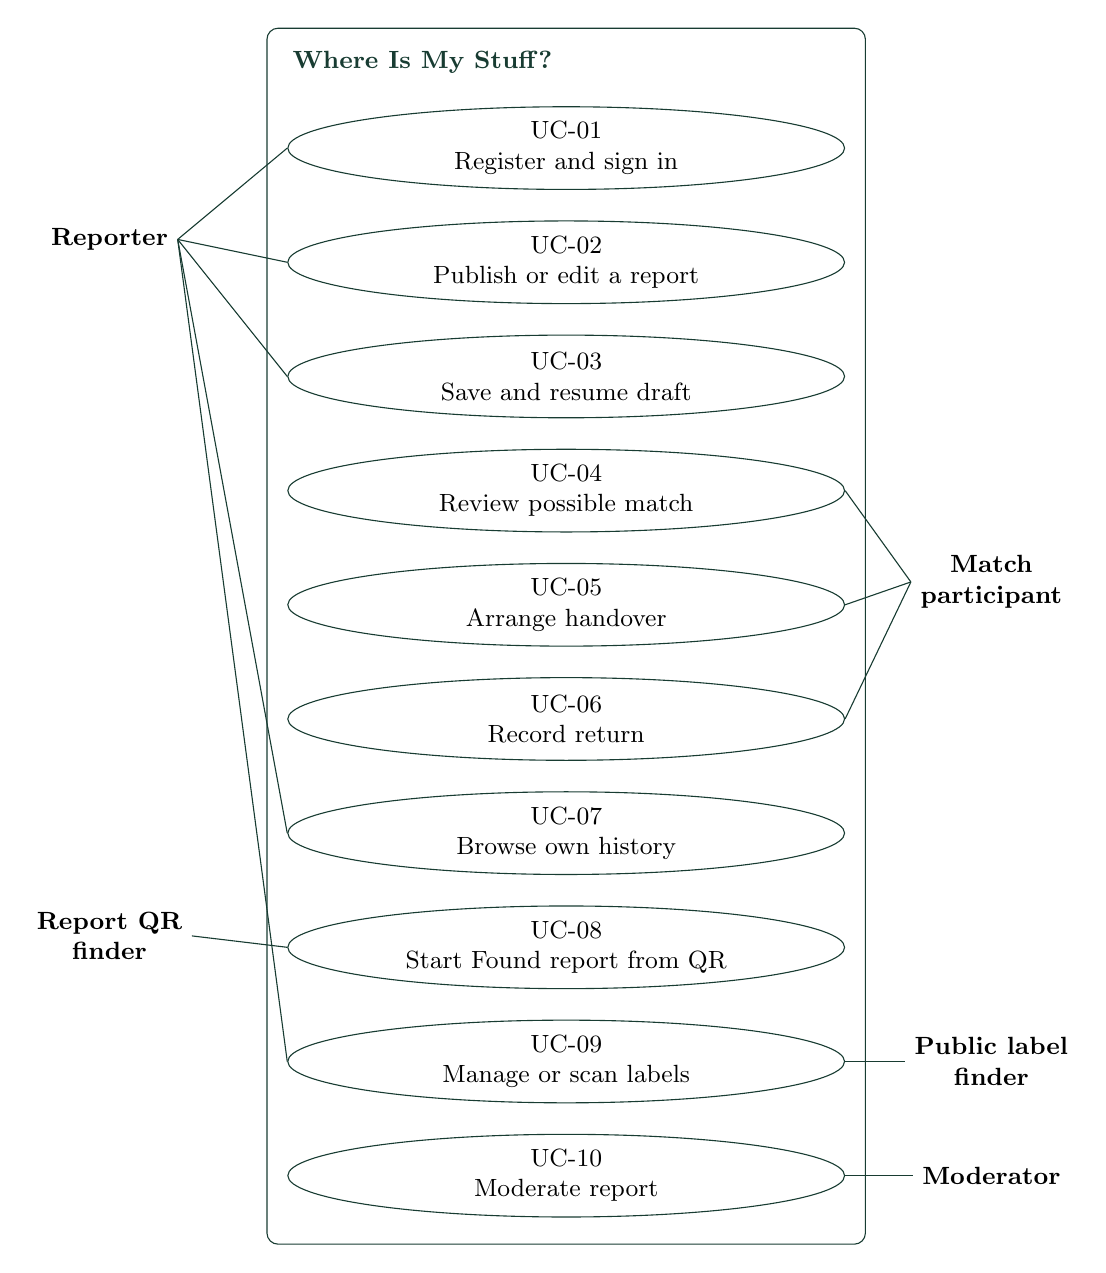
\begin{tikzpicture}[x=1cm,y=1.45cm,uc/.style={ellipse,draw=ink,minimum width=6.5cm,minimum height=1.05cm,inner sep=0pt,text width=5cm,align=center,font=\small},actor/.style={align=center,font=\small\bfseries}]
\draw[rounded corners,draw=ink] (3,-.6) rectangle (10.6,10.05);
\node[anchor=west,font=\small\bfseries,color=ink] at (3.2,9.75) {Where Is My Stuff?};
\foreach \y/\id/\txt in {9/01/Register and sign in,8/02/Publish or edit a report,7/03/Save and resume draft,6/04/Review possible match,5/05/Arrange handover,4/06/Record return,3/07/Browse own history,2/08/Start Found report from QR,1/09/Manage or scan labels,0/10/Moderate report}
{\node[uc] (u\id) at (6.8,\y) {UC-\id\\\txt};}
\node[actor] (reporter) at (1,8.2) {Reporter};
\node[actor] (participant) at (12.2,5.2) {Match\\participant};
\node[actor] (finder) at (1,2.1) {Report QR\\finder};
\node[actor] (public) at (12.2,1.0) {Public label\\finder};
\node[actor] (staff) at (12.2,0) {Moderator};
\foreach \id in {01,02,03,07,09} {\draw[draw=ink] (reporter.east)--(u\id.west);}
\foreach \id in {04,05,06} {\draw[draw=ink] (participant.west)--(u\id.east);}
\draw[draw=ink] (finder.east)--(u08.west);
\draw[draw=ink] (public.west)--(u09.east);
\draw[draw=ink] (staff.west)--(u10.east);
\end{tikzpicture}
\caption{Use case view. Textual actor symbols identify the external roles; UC-09 includes owner management and public scanning.}
\end{figure}

\begin{longtable}{@{}P{0.26\dimexpr\textwidth-12pt\relax}P{0.74\dimexpr\textwidth-12pt\relax}@{}}

\toprule \textbf{ID / actor} & \textbf{Brief use case description} \\ \midrule\endfirsthead

\toprule \textbf{ID / actor} & \textbf{Brief use case description} \\ \midrule\endhead

\bottomrule\endfoot

UC-01 / Reporter & Register with unique email or authenticate; create a session and enter the report/dashboard flow. Invalid credentials or password validation failure produces an error. \\ \addlinespace[3pt]

UC-02 / Reporter & Complete all report stages, review and publish. Revalidate every field, write the report/event, calculate matches and remove the draft. An owner can edit only Open, unreserved reports. \\ \addlinespace[3pt]

UC-03 / Reporter & Submit a valid stage, leave and resume saved data. Explicit confirmation is required when discarding a draft through the normal new-report workflow. \\ \addlinespace[3pt]

UC-04 / Match participant & Open a permitted match; compare both public summaries and factor points. Private answers remain hidden; a score is not proof of ownership. \\ \addlinespace[3pt]

UC-05 / Match participant & Propose a future meeting; reserve both reports; let the other participant accept. Either may dismiss a possible/proposed match; only the dismisser may restore an eligible pair. \\ \addlinespace[3pt]

UC-06 / Match participant & At or after the scheduled time, record return. Update both reports, release reservations, reject competing possible matches and write events. \\ \addlinespace[3pt]

UC-07 / Reporter & Browse own report summaries, search title/place, filter kind/status and paginate history. Removed records are absent from ordinary lists. \\ \addlinespace[3pt]

UC-08 / Signed-in report QR finder & Open a UUID link, seed/reuse a Found draft with limited public hints, then independently complete the report. Self-use redirects; closed/reserved sources show a notice. \\ \addlinespace[3pt]

UC-09 / Owner / public label finder & Owner creates/downloads/deactivates/reactivates a label. A bearer URL shows the chosen phone only while the label is active; an unknown token is not found. \\ \addlinespace[3pt]

UC-10 / Moderator & Inspect the staff list and close/remove an Open unreserved report. Reject related possible matches and record the staff action; deny nonstaff access. \\ \addlinespace[3pt]

\end{longtable}

These brief descriptions follow the supplied format; detailed step-by-step test procedures belong in a separate test plan. Administrator account management is a supporting framework function, outside UC-01 to UC-10.

\Needspace{12\baselineskip}

\subsection{Report and Handover State Models}

\begin{figure}[H]\centering

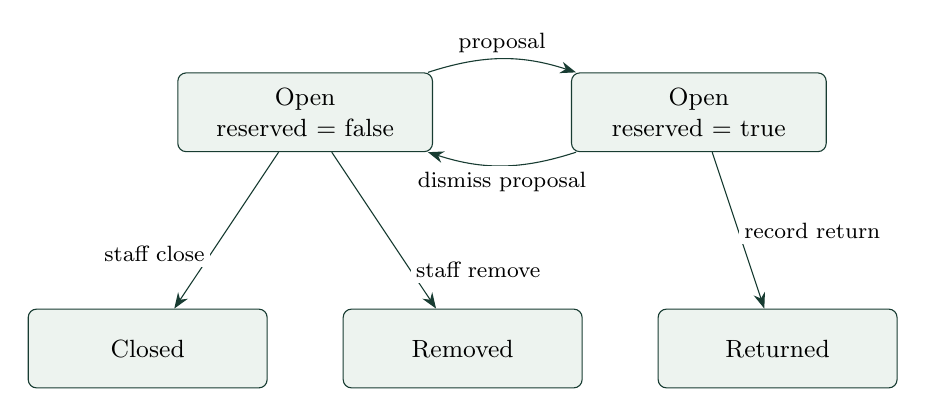
\begin{tikzpicture}
\node[box,text width=3cm] (open) at (-2,2) {Open\\reserved = false};
\node[box,text width=3cm] (reserved) at (3,2) {Open\\reserved = true};
\node[box,text width=2.8cm] (closed) at (-4,-1) {Closed};
\node[box,text width=2.8cm] (removed) at (0,-1) {Removed};
\node[box,text width=2.8cm] (returned) at (4,-1) {Returned};
\draw[arr] (open) to[bend left=18] node[lab,above]{proposal}(reserved);
\draw[arr] (reserved) to[bend left=18] node[lab,below]{dismiss proposal}(open);
\draw[arr] (open)--node[lab,left,pos=.65]{staff close}(closed);
\draw[arr] (open)--node[lab,right,pos=.75]{staff remove}(removed);
\draw[arr] (reserved)--node[lab,right]{record return}(returned);
\end{tikzpicture}
\caption{Report status and reservation. Reserved is a separate Boolean, not a report status.}
\end{figure}
\begin{figure}[H]\centering
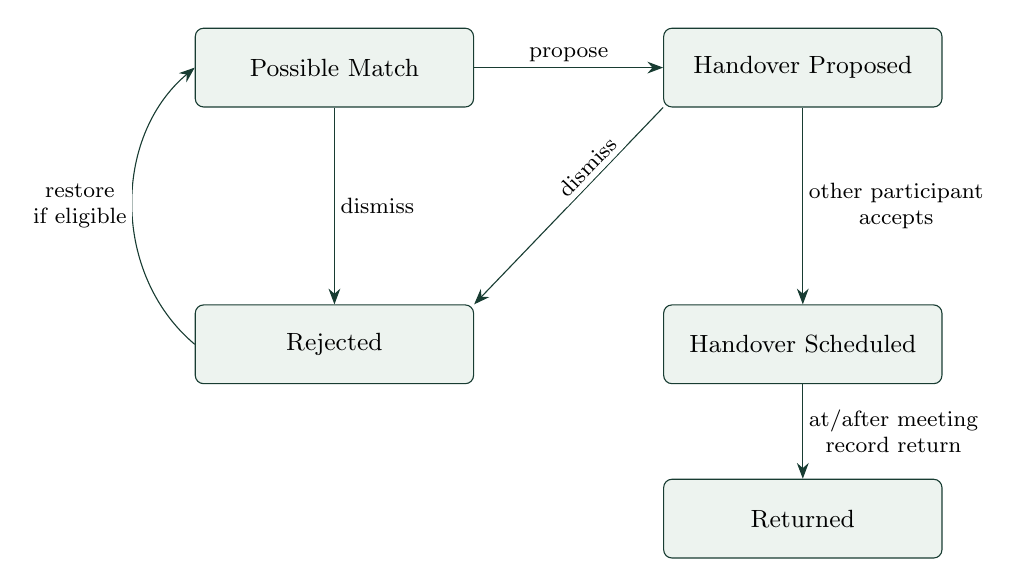
\begin{tikzpicture}[node distance=1.0cm and 1.1cm]
\node[box] (possible) {Possible Match};
\node[box,right=2.4cm of possible] (proposed) {Handover Proposed};
\node[box,below=2.5cm of proposed] (scheduled) {Handover Scheduled};
\node[box,left=2.4cm of scheduled] (rejected) {Rejected};
\node[box,below=1.2cm of scheduled] (returned) {Returned};
\draw[arr] (possible)--node[lab,above]{propose}(proposed);
\draw[arr] (proposed)--node[lab,right]{other participant\\accepts}(scheduled);
\draw[arr] (scheduled)--node[lab,right]{at/after meeting\\record return}(returned);
\draw[arr] (possible.south) -- node[lab,right]{dismiss}(rejected.north);
\draw[arr] (rejected.west) to[bend left=50] node[lab,left]{restore\\if eligible}(possible.west);
\draw[arr] (proposed.south west)--node[lab,above,sloped,pos=.35]{dismiss}(rejected.north east);
\end{tikzpicture}
\caption{Match lifecycle. Staff closure/removal and competing return also reject related Possible Match records.}
\end{figure}

\begin{longtable}{@{}P{0.19\dimexpr\textwidth-12pt\relax}P{0.81\dimexpr\textwidth-12pt\relax}@{}}

\toprule \textbf{Action} & \textbf{Guards and effects} \\ \midrule\endfirsthead

\toprule \textbf{Action} & \textbf{Guards and effects} \\ \midrule\endhead

\bottomrule\endfoot

Propose & Participant; Possible Match; both reports Open and unreserved; valid future meeting. Sets both reserved, records proposer/place/time and proposed state. \\ \addlinespace[3pt]

Accept & Other participant; Handover Proposed; meeting remains in future; reports Open. Sets scheduled state; reveals contacts. \\ \addlinespace[3pt]

Dismiss & Either participant; Possible Match or Handover Proposed; reports Open. Sets Rejected and rejected\_by. A dismissed proposal releases both reservations. \\ \addlinespace[3pt]

Restore & Only rejected\_by; reports Open and unreserved; current score still qualifies. Sets Possible Match and refreshes scores; clears rejected\_by. \\ \addlinespace[3pt]

Return & Either participant; Handover Scheduled; meeting time reached; reports Open. Sets both Returned, clears reservations and rejects competing Possible Match records. \\ \addlinespace[3pt]

Close / remove & Staff only; report Open and unreserved. Sets Closed/Removed, rejects related possible matches and records an event. \\ \addlinespace[3pt]

\end{longtable}

\Needspace{12\baselineskip}

\subsection{Publication Interaction Model}

\begin{figure}[H]\centering
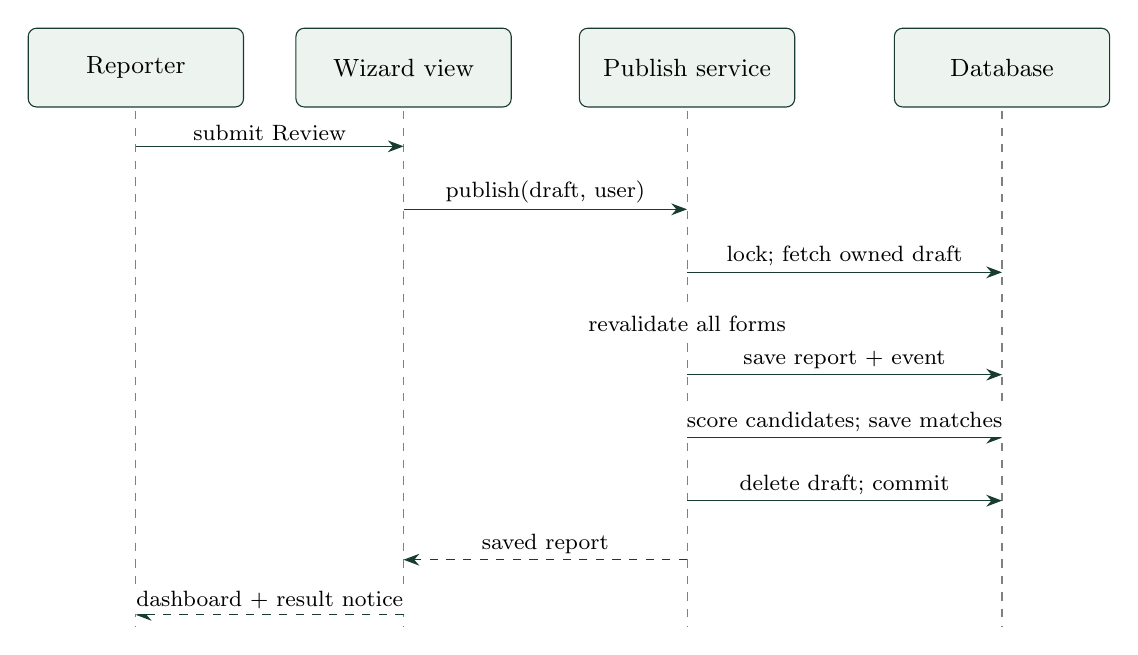
\begin{tikzpicture}[x=1cm,y=1cm]
\foreach \x/\n/\t in {0/u/Reporter,3.4/v/Wizard view,7/s/Publish service,11/d/Database}
{\node[box,text width=2.5cm] (\n) at (\x,0) {\t};\draw[dashed,gray] (\x,-.55)--(\x,-7.1);}
\draw[arr] (0,-1)--node[lab,above]{submit Review}(3.4,-1);
\draw[arr] (3.4,-1.8)--node[lab,above]{publish(draft, user)}(7,-1.8);
\draw[arr] (7,-2.6)--node[lab,above]{lock; fetch owned draft}(11,-2.6);
\node[lab] at (7,-3.25) {revalidate all forms};
\draw[arr] (7,-3.9)--node[lab,above]{save report + event}(11,-3.9);
\draw[arr] (7,-4.7)--node[lab,above]{score candidates; save matches}(11,-4.7);
\draw[arr] (7,-5.5)--node[lab,above]{delete draft; commit}(11,-5.5);
\draw[arr,dashed] (7,-6.25)--node[lab,above]{saved report}(3.4,-6.25);
\draw[arr,dashed] (3.4,-6.95)--node[lab,above]{dashboard + result notice}(0,-6.95);
\end{tikzpicture}
\caption{Successful publication. Validation failure returns an error; transactional database changes do not partially commit.}
\end{figure}

\Needspace{12\baselineskip}

\subsection{Business Rules and Matching Calculation}

\begin{longtable}{@{}P{0.15\dimexpr\textwidth-12pt\relax}P{0.85\dimexpr\textwidth-12pt\relax}@{}}

\toprule \textbf{ID} & \textbf{Rule} \\ \midrule\endfirsthead

\toprule \textbf{ID} & \textbf{Rule} \\ \midrule\endhead

\bottomrule\endfoot

BR-01 & A report, match or QR scan is a lead only. Only a valid participant return action sets the matched reports to Returned. \\ \addlinespace[3pt]

BR-02 & The five score factors total at most 100. Threshold 70 and at least two meaningful private agreements are both mandatory. \\ \addlinespace[3pt]

BR-03 & Scoring accepts only Lost-to-Found, same-category, Open reports from different owners. Candidate retrieval excludes reserved reports. \\ \addlinespace[3pt]

BR-04 & A proposed or scheduled handover reserves both reports and blocks editing, moderation and competing proposals. \\ \addlinespace[3pt]

BR-05 & The report remains Open while reserved. Closed, Removed and Returned reports cannot receive normal editing or handover actions. \\ \addlinespace[3pt]

BR-06 & Report contacts become visible to participants after acceptance and stay visible after return. Active personal labels separately publish their chosen phone. \\ \addlinespace[3pt]

BR-07 & Recalculation deletes existing Possible Match rows involving the edited/published report before rebuilding suggestions. Existing rejected/proposed/scheduled pair states are not reset to Possible Match. \\ \addlinespace[3pt]

BR-08 & Event entries are created for report creation/update, match transitions and moderation. Match score generation itself is not a separately logged Event. \\ \addlinespace[3pt]

\end{longtable}

\begin{longtable}{@{}P{0.19\dimexpr\textwidth-24pt\relax}P{0.14\dimexpr\textwidth-24pt\relax}P{0.67\dimexpr\textwidth-24pt\relax}@{}}

\toprule \textbf{Factor} & \textbf{Maximum} & \textbf{Calculation} \\ \midrule\endfirsthead

\toprule \textbf{Factor} & \textbf{Maximum} & \textbf{Calculation} \\ \midrule\endhead

\bottomrule\endfoot

Category & 20 & Exact category equality; otherwise the pair is ineligible. \\ \addlinespace[3pt]

Location & 20 & Haversine distance: below 0.5 km = 20; below 1 km = 15; below 2 km = 10; below 5 km = 5; otherwise 0. Missing coordinates give 0. \\ \addlinespace[3pt]

Date & 15 & Absolute event-date difference: 0 days = 15; 1 day = 10; 2-3 days = 5; otherwise 0. \\ \addlinespace[3pt]

Description & 15 & Casefold text; extract [a-z0-9] tokens of length at least 3; remove configured stop words. Round 15 times intersection size / union size. Empty union gives 0. \\ \addlinespace[3pt]

Private & 30 & Normalize ordinary values by stripping and casefolding. Count agreements over the union of evidence keys plus bank-card pairs. Round 30 times agreements / evidence total. Empty total gives 0. \\ \addlinespace[3pt]

\end{longtable}

Private evidence excludes contents, bank\_count and logo selectors, all bank\_* keys from ordinary key comparisons, and values None, empty string, "None", "Other", "Not provided", empty list and "No". Conditional logo\_name and other filled descriptive fields can contribute. Bank-card entries are compared as a set of (issuer or custom service, complete number stored in *\_suffix) pairs, independent of entry order. Each identical pair contributes one agreement. Ordinary matching fields include generic colour/type as well as more distinctive details; two agreements do not establish ownership.

Description stop words are: the, and, with, from, near, was, for, this, that, have, item, lost, found. Python round is used for fractional description/private scores. At exactly 0.5, 1, 2 or 5 km the lower distance band no longer applies. A hypothetical pair with 20 category + 10 location + 10 date + 10 description + 20 private = 70 qualifies only if at least two private agreements also exist.

\chapter{Other Non-functional Requirements}

\Needspace{14\baselineskip}

\section{Performance Requirements}

The following five measurable targets are Proposed. They complete the performance specification requested by the course template; they are not measured achievements. Reference workload: 1,000 Open reports, 10 concurrent authenticated users, 2-vCPU/4-GiB server with SSD, PostgreSQL, warm cache and same-region client network. Measure p95 over at least 100 operations after warm-up. Exclude external map-tile latency; include database and server work. Record hardware and test data when approving the targets.

\Needspace{6\baselineskip}\noindent\begin{minipage}{\linewidth}\textbf{NFR-PER-01}\hfill\textit{Medium}\par\nopagebreak

Proposed: Ordinary dashboard, history and detail page loads shall complete within 2 seconds at p95.

{\color{muted}\textbf{Acceptance:} Measure browser navigation through load completion under the reference workload.\par}\end{minipage}\par\vspace{5pt}

\Needspace{6\baselineskip}\noindent\begin{minipage}{\linewidth}\textbf{NFR-PER-02}\hfill\textit{Medium}\par\nopagebreak

Proposed: Report publication including candidate matching shall complete within 5 seconds at p95.

{\color{muted}\textbf{Acceptance:} Measure submit-to-redirect completion for representative reports, including the largest same-category candidate set.\par}\end{minipage}\par\vspace{5pt}

\Needspace{6\baselineskip}\noindent\begin{minipage}{\linewidth}\textbf{NFR-PER-03}\hfill\textit{Medium}\par\nopagebreak

Proposed: Valid wizard-step submissions without a photo shall complete within 1 second at p95.

{\color{muted}\textbf{Acceptance:} Measure POST-to-next-step response; confirm data has persisted before the next step is shown.\par}\end{minipage}\par\vspace{5pt}

\Needspace{6\baselineskip}\noindent\begin{minipage}{\linewidth}\textbf{NFR-PER-04}\hfill\textit{Medium}\par\nopagebreak

Proposed: Photo validation and normalization at the allowed 5-MiB/24-megapixel boundary shall finish within 3 seconds at p95 after upload receipt.

{\color{muted}\textbf{Acceptance:} Time decode, normalize and private-storage write for valid boundary images; exclude client upload transfer.\par}\end{minipage}\par\vspace{5pt}

\Needspace{6\baselineskip}\noindent\begin{minipage}{\linewidth}\textbf{NFR-PER-05}\hfill\textit{Medium}\par\nopagebreak

Proposed: Personal-label creation including QR generation shall finish within 2 seconds at p95.

{\color{muted}\textbf{Acceptance:} Measure successful POST through persisted label and available image with 10 concurrent users.\par}\end{minipage}\par\vspace{5pt}

\Needspace{14\baselineskip}

\section{Safety and Security Requirements}

\Needspace{12\baselineskip}

\subsection{Safety and Trust}

\Needspace{6\baselineskip}\noindent\begin{minipage}{\linewidth}\textbf{SAFE-01}\hfill\textit{High}\par\nopagebreak

Match and QR interfaces shall explain that the application does not establish ownership or guarantee recovery.

{\color{muted}\textbf{Acceptance:} Match/report QR screens display the limitation; no automatic ownership claim is made.\par}\end{minipage}\par\vspace{5pt}

\Needspace{6\baselineskip}\noindent\begin{minipage}{\linewidth}\textbf{SAFE-02}\hfill\textit{High}\par\nopagebreak

The handover form shall guide users to choose a public, safe meeting place.

{\color{muted}\textbf{Acceptance:} Meeting-place help contains the guidance. This is advice; the system does not assess the safety of a location.\par}\end{minipage}\par\vspace{5pt}

\Needspace{6\baselineskip}\noindent\begin{minipage}{\linewidth}\textbf{SAFE-03}\hfill\textit{High}\par\nopagebreak

The system shall prevent return confirmation before the scheduled time and prevent overlapping active handovers for a report.

{\color{muted}\textbf{Acceptance:} Early return and competing proposals are refused without changing report state.\par}\end{minipage}\par\vspace{5pt}

\Needspace{12\baselineskip}

\subsection{Security and Privacy}

\Needspace{6\baselineskip}\noindent\begin{minipage}{\linewidth}\textbf{NFR-SEC-01}\hfill\textit{High}\par\nopagebreak

Restricted application pages shall require a valid authenticated session.

{\color{muted}\textbf{Acceptance:} Anonymous requests redirect to login or return no protected content.\par}\end{minipage}\par\vspace{5pt}

\Needspace{6\baselineskip}\noindent\begin{minipage}{\linewidth}\textbf{NFR-SEC-02}\hfill\textit{High}\par\nopagebreak

Authorization shall be checked against the object owner, match participation or staff role.

{\color{muted}\textbf{Acceptance:} Cross-account report/draft/match/media access is denied. Staff permission alone does not grant photo or private-answer access.\par}\end{minipage}\par\vspace{5pt}

\Needspace{6\baselineskip}\noindent\begin{minipage}{\linewidth}\textbf{NFR-SEC-03}\hfill\textit{High}\par\nopagebreak

State-changing POST forms shall use CSRF protection.

{\color{muted}\textbf{Acceptance:} Missing/invalid tokens reject POST submission. GET draft mutations remain a known gap in Chapter 5.\par}\end{minipage}\par\vspace{5pt}

\Needspace{6\baselineskip}\noindent\begin{minipage}{\linewidth}\textbf{NFR-SEC-04}\hfill\textit{High}\par\nopagebreak

The server shall revalidate current state and reservation at action time.

{\color{muted}\textbf{Acceptance:} A stale form cannot edit, moderate or propose against an ineligible report.\par}\end{minipage}\par\vspace{5pt}

\Needspace{6\baselineskip}\noindent\begin{minipage}{\linewidth}\textbf{NFR-SEC-05}\hfill\textit{High}\par\nopagebreak

Other users and staff management pages shall not receive raw private answers.

{\color{muted}\textbf{Acceptance:} Inspect report/match/management responses for absence of the other owner's answers. This is application access control, not encryption against database administrators.\par}\end{minipage}\par\vspace{5pt}

\Needspace{6\baselineskip}\noindent\begin{minipage}{\linewidth}\textbf{NFR-SEC-06}\hfill\textit{High}\par\nopagebreak

Production secrets shall be supplied through protected deployment configuration.

{\color{muted}\textbf{Acceptance:} Production configuration rejects missing/weak required settings; a separate release review checks distributable files for secrets.\par}\end{minipage}\par\vspace{5pt}

\Needspace{6\baselineskip}\noindent\begin{minipage}{\linewidth}\textbf{NFR-SEC-07}\hfill\textit{High}\par\nopagebreak

Proposed deployment gate: approve collection, minimization, retention and deletion rules for private identifiers, photos and contact data.

{\color{muted}\textbf{Acceptance:} A documented policy identifies permitted fields, retention periods, access roles and deletion procedures before public use.\par}\end{minipage}\par\vspace{5pt}

\Needspace{6\baselineskip}\noindent\begin{minipage}{\linewidth}\textbf{NFR-SEC-08}\hfill\textit{High}\par\nopagebreak

Report photos, draft photos and personal-label images shall use authorization-aware responses with private, no-store caching.

{\color{muted}\textbf{Acceptance:} Authorized media includes required headers; unrelated users receive no image bytes. Public report QR PNGs are a separate non-photo endpoint.\par}\end{minipage}\par\vspace{5pt}

\begin{longtable}{@{}P{0.19\dimexpr\textwidth-12pt\relax}P{0.81\dimexpr\textwidth-12pt\relax}@{}}

\toprule \textbf{Security rule} & \textbf{Specification / acceptance reference} \\ \midrule\endfirsthead

\toprule \textbf{Security rule} & \textbf{Specification / acceptance reference} \\ \midrule\endhead

\bottomrule\endfoot

SEC-01 & Object scope is defined by NFR-SEC-02 and the disclosure matrix in Chapter 5. \\ \addlinespace[3pt]

SEC-02 & Both saved report contacts remain hidden until the other participant accepts; compare responses before and after acceptance (FR-HND-05/06). \\ \addlinespace[3pt]

SEC-03 & Report QR hints omit the source phone, private answers, exact coordinates and location description (FR-QR-02/03). \\ \addlinespace[3pt]

SEC-04 & Label token\_hash is a digest; inactive labels omit the phone. The QR image contains the bearer URL (FR-QR-06/08). \\ \addlinespace[3pt]

SEC-05 & Decode and re-encode photos, remove source metadata, enforce size/type/dimensions and restrict access; no photo similarity analysis (FR-PHO). \\ \addlinespace[3pt]

SEC-06 & Public deployment shall use HTTPS, secure cookies, explicit hosts, protected secrets and production headers. Verify against config/production.py and actual deployment. \\ \addlinespace[3pt]

SEC-07 & Trust notices shall communicate application limits (SAFE-01/02). \\ \addlinespace[3pt]

SEC-08 & Apply configured identifier and invisible-character filters to public text (FR-VAL-01/02). These pattern filters are not a complete personal-data detector. \\ \addlinespace[3pt]

\end{longtable}

Some private forms request complete 13-digit CNIC and 16-digit card numbers despite keys named suffix. These values are stored in JSON without additional field encryption. Password-style inputs mask rendering but do not change storage. This fact must remain explicit in the specification and any decision about public deployment.

\Needspace{14\baselineskip}

\section{Software Quality Attributes}

\Needspace{12\baselineskip}

\subsection{Reliability and Data Integrity}

\Needspace{6\baselineskip}\noindent\begin{minipage}{\linewidth}\textbf{NFR-REL-01}\hfill\textit{High}\par\nopagebreak

Publishing, recalculating matches, moderation and handover transitions shall commit database changes atomically.

{\color{muted}\textbf{Acceptance:} An induced database failure shall leave no partial workflow state. Filesystem writes are not claimed to share the database transaction.\par}\end{minipage}\par\vspace{5pt}

\Needspace{6\baselineskip}\noindent\begin{minipage}{\linewidth}\textbf{NFR-REL-02}\hfill\textit{High}\par\nopagebreak

At most one active handover shall reserve a report.

{\color{muted}\textbf{Acceptance:} Concurrent proposal scenarios shall produce one reservation winner and rejection of a competing proposal.\par}\end{minipage}\par\vspace{5pt}

\Needspace{6\baselineskip}\noindent\begin{minipage}{\linewidth}\textbf{NFR-REL-03}\hfill\textit{High}\par\nopagebreak

A Lost/Found pair shall be unique and match score shall not exceed 100.

{\color{muted}\textbf{Acceptance:} Database unique\_pair and score\_maximum constraints reject invalid inserts.\par}\end{minipage}\par\vspace{5pt}

\Needspace{6\baselineskip}\noindent\begin{minipage}{\linewidth}\textbf{NFR-REL-04}\hfill\textit{High}\par\nopagebreak

Schema changes shall use versioned migrations.

{\color{muted}\textbf{Acceptance:} Clean installation and upgrade shall reach migrations 0001-0006 without manual schema edits.\par}\end{minipage}\par\vspace{5pt}

\Needspace{12\baselineskip}

\subsection{Usability and Accessibility}

\Needspace{6\baselineskip}\noindent\begin{minipage}{\linewidth}\textbf{NFR-USE-01}\hfill\textit{Medium}\par\nopagebreak

Proposed: at least 8 of 10 first-time participants shall publish a valid report without assistance, with median completion within 5 minutes.

{\color{muted}\textbf{Acceptance:} Observe a defined representative task and report success rate and median elapsed time.\par}\end{minipage}\par\vspace{5pt}

\Needspace{6\baselineskip}\noindent\begin{minipage}{\linewidth}\textbf{NFR-USE-02}\hfill\textit{Medium}\par\nopagebreak

Core form fields shall have labels and validation errors that indicate corrective action.

{\color{muted}\textbf{Acceptance:} Inspect account, wizard, meeting and label forms for labels and actionable errors.\par}\end{minipage}\par\vspace{5pt}

\Needspace{6\baselineskip}\noindent\begin{minipage}{\linewidth}\textbf{NFR-USE-03}\hfill\textit{Medium}\par\nopagebreak

Users shall be able to enter place text and coordinates when external map tiles are unavailable.

{\color{muted}\textbf{Acceptance:} Complete Location with manual fields while tile requests fail.\par}\end{minipage}\par\vspace{5pt}

\Needspace{6\baselineskip}\noindent\begin{minipage}{\linewidth}\textbf{NFR-ACC-01}\hfill\textit{Medium}\par\nopagebreak

Proposed: core flows shall satisfy WCAG 2.2 AA requirements for keyboard use, focus, labels, contrast and error identification.

{\color{muted}\textbf{Acceptance:} A documented manual and automated accessibility audit records conformance and remaining failures.\par}\end{minipage}\par\vspace{5pt}

\Needspace{12\baselineskip}

\subsection{Compatibility and Localization}

\Needspace{6\baselineskip}\noindent\begin{minipage}{\linewidth}\textbf{NFR-COMP-01}\hfill\textit{Medium}\par\nopagebreak

Proposed: core workflows shall work in current and previous major Chrome, Edge, Firefox and Safari, with defined desktop/mobile versions.

{\color{muted}\textbf{Acceptance:} Execute an approved browser matrix. The Appendix C observation covers Chrome only.\par}\end{minipage}\par\vspace{5pt}

\Needspace{6\baselineskip}\noindent\begin{minipage}{\linewidth}\textbf{NFR-LOC-01}\hfill\textit{Medium}\par\nopagebreak

Dates and meetings shall use Asia/Karachi for interpretation and display; persistent datetime values shall be timezone aware.

{\color{muted}\textbf{Acceptance:} Save a meeting and compare its displayed Pakistan time with the stored instant.\par}\end{minipage}\par\vspace{5pt}

\Needspace{12\baselineskip}

\subsection{Maintainability and Testability}

\Needspace{6\baselineskip}\noindent\begin{minipage}{\linewidth}\textbf{NFR-MNT-01}\hfill\textit{Medium}\par\nopagebreak

Matching, transitions and moderation shall remain callable independently of template rendering.

{\color{muted}\textbf{Acceptance:} Service functions can be exercised with model fixtures without opening a browser.\par}\end{minipage}\par\vspace{5pt}

\Needspace{6\baselineskip}\noindent\begin{minipage}{\linewidth}\textbf{NFR-MNT-02}\hfill\textit{Medium}\par\nopagebreak

All baseline functional requirements shall have mapped acceptance scenarios before release approval.

{\color{muted}\textbf{Acceptance:} Appendix B maps every FR family; a release test record shall add individual results and evidence.\par}\end{minipage}\par\vspace{5pt}

\Needspace{12\baselineskip}

\subsection{Availability and Recoverability}

\Needspace{6\baselineskip}\noindent\begin{minipage}{\linewidth}\textbf{NFR-OPS-01}\hfill\textit{Medium}\par\nopagebreak

Proposed: production database and private-media backups shall run daily, retain 14 daily recovery points and be restored in a quarterly exercise with recovery-point loss at most 24 hours.

{\color{muted}\textbf{Acceptance:} Restore database and referenced files together and record recovery evidence.\par}\end{minipage}\par\vspace{5pt}

\Needspace{6\baselineskip}\noindent\begin{minipage}{\linewidth}\textbf{NFR-OPS-02}\hfill\textit{Medium}\par\nopagebreak

Proposed: public service availability shall be at least 99.5\% per calendar month, excluding announced maintenance.

{\color{muted}\textbf{Acceptance:} Use timestamped availability monitoring over the complete month.\par}\end{minipage}\par\vspace{5pt}

Correctness, privacy and workflow integrity take priority over convenience and performance. Database schema, matching rules and views are separate modules to support changes. New questionnaire fields require corresponding validation, scoring, privacy and data-dictionary updates rather than a UI-only change.

\chapter{Other Requirements}

\Needspace{14\baselineskip}

\section{Database Tables and Relationships}

The six application tables are core\_user, core\_report, core\_draft, core\_match, core\_event and core\_qrlabel. Django additionally maintains authentication, permission, session, content-type, administration-log and migration tables. The application field dictionary appears in Appendix A. JSON is used for category-varying answers and draft data; it is not a separate relational table.

\begin{figure}[H]\centering
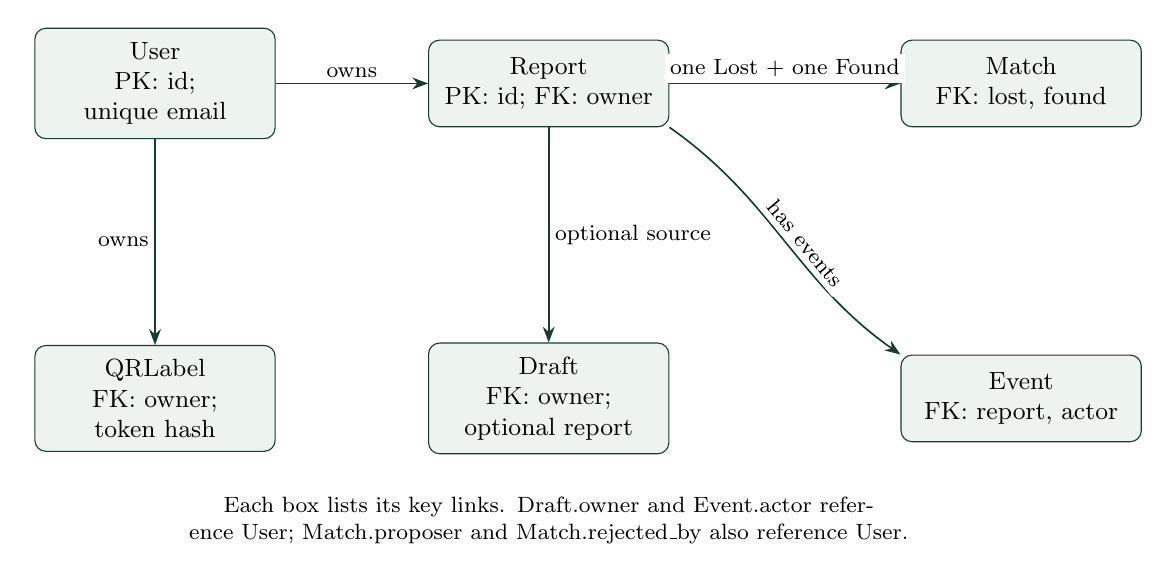
\begin{tikzpicture}[x=1cm,y=1cm,
  entity/.style={draw=ink,rounded corners=4pt,fill=pale,align=center,
    text width=2.7cm,minimum height=1.1cm,inner sep=5pt,font=\small},
  relation/.style={-{Stealth[length=2mm]},draw=ink,line width=.6pt},
  relabel/.style={font=\footnotesize,fill=white,inner sep=2pt,align=center}]
\node[entity] (user) at (0,2) {User\\PK: id; unique email};
\node[entity] (report) at (5,2) {Report\\PK: id; FK: owner};
\node[entity] (match) at (11,2) {Match\\FK: lost, found};
\node[entity] (label) at (0,-2) {QRLabel\\FK: owner; token hash};
\node[entity] (draft) at (5,-2) {Draft\\FK: owner; optional report};
\node[entity] (event) at (11,-2) {Event\\FK: report, actor};
\draw[relation] (user.east)--node[relabel,above]{owns}(report.west);
\draw[relation] (report.east)--node[relabel,above]{one Lost + one Found}(match.west);
\draw[relation] (user.south)--node[relabel,left]{owns}(label.north);
\draw[relation] (report.south)--node[relabel,right]{optional source}(draft.north);
\draw[relation] (report.south east) to[out=-35,in=145] node[relabel,sloped,above,pos=.55]{has events} (event.north west);
\node[font=\footnotesize,align=center,text width=13cm] at (5,-3.55)
  {Each box lists its key links. Draft.owner and Event.actor reference User; Match.proposer and Match.rejected\_by also reference User.};
\end{tikzpicture}
\caption{Application entities and their principal relationships.}
\end{figure}

\begin{itemize}

\item Every report has one protected owner. Match.lost, Match.found, Match.proposer, Match.rejected\_by and Event references use PROTECT deletion behavior.

\item Draft and QRLabel owner links use CASCADE; Draft.report is nullable and cascades if its source report is deleted. Normal moderation sets status rather than physically deleting reports.

\item Match(lost, found) is unique; score is a positive small integer constrained to at most 100. Report.public\_id and QRLabel.token\_hash are unique.

\item Only kind has model choices on Report. Status and state are string fields controlled by service logic; no additional database state-enumeration or one-active-handover constraint is declared.

\item The service locks an owner row to avoid duplicate creation of a new draft in normal concurrent requests. Historical duplicates can still exist; the newest matching draft is resumed.

\item Framework tables include core\_user\_groups, core\_user\_user\_permissions, auth\_group, auth\_permission, auth\_group\_permissions, django\_session, django\_content\_type, django\_admin\_log and django\_migrations.

\end{itemize}

\Needspace{14\baselineskip}

\section{Data Disclosure and Retention}

\begin{longtable}{@{}P{0.26\dimexpr\textwidth-12pt\relax}P{0.74\dimexpr\textwidth-12pt\relax}@{}}

\toprule \textbf{Data} & \textbf{Permitted application visibility} \\ \midrule\endfirsthead

\toprule \textbf{Data} & \textbf{Permitted application visibility} \\ \midrule\endhead

\bottomrule\endfoot

Owned report and draft & Owner. Match views reveal the paired report's public summary; the standalone report detail route stays owner-only. \\ \addlinespace[3pt]

Private answers & Owner during authorized draft entry/editing; server for scoring. Absent from the opposite participant's output and staff management. Administrators with database access are outside this UI protection. \\ \addlinespace[3pt]

Report contact phone & Owner during Details entry; both match participants after the other party accepts (scheduled/returned states). Not exposed by the report QR seed. \\ \addlinespace[3pt]

Report photo & Owner and owner of the opposite report in any existing match involving it. The current photo query does not exclude Rejected matches. \\ \addlinespace[3pt]

Draft photo & Draft owner only. \\ \addlinespace[3pt]

Report QR PNG & Public to anyone holding the UUID URL; contains only the entry URL. Following it requires authentication before seeding a draft. \\ \addlinespace[3pt]

Personal QR image & Owner only. It encodes a bearer URL; a shared printed image grants scan capability. \\ \addlinespace[3pt]

Personal-label phone & Anyone with the bearer URL while active. Suppressed when expired/revoked; no login is required for public scanning. \\ \addlinespace[3pt]

Activity event & Stored actor, text and time. Owner report UI shows text/time; management actions are attributable in the database. \\ \addlinespace[3pt]

\end{longtable}

There is no automatic retention schedule, user deletion/export workflow or account recovery workflow in this baseline. Label expiry disables public contact display; it does not delete the label record or image. Removing a report is a status change and is not erasure. These distinctions must be considered when defining production retention policy.

\Needspace{14\baselineskip}

\section{Known Limitations and Open Decisions}

\begin{longtable}{@{}P{0.15\dimexpr\textwidth-12pt\relax}P{0.85\dimexpr\textwidth-12pt\relax}@{}}

\toprule \textbf{ID} & \textbf{Observed behavior / decision} \\ \midrule\endfirsthead

\toprule \textbf{ID} & \textbf{Observed behavior / decision} \\ \midrule\endhead

\bottomrule\endfoot

OI-01 & Private questionnaires store complete CNIC/card values without field encryption. Decide whether these fields are necessary and define minimization, retention and deletion before public deployment. \\ \addlinespace[3pt]

OI-02 & Approve reference hardware, quality thresholds and operational targets before treating Proposed requirements as release gates. \\ \addlinespace[3pt]

GAP-01 & The private-identifier validation hint incorrectly says the matched party sees private answers; templates actually suppress them. UI wording should be aligned to the privacy model. \\ \addlinespace[3pt]

GAP-02 & New-report and report-QR GET routes can create or modify a draft. CSRF guarantees in this document apply to POST forms; moving draft mutations behind confirmed POST requests is a follow-up change. \\ \addlinespace[3pt]

GAP-03 & Report QR entry reuses the newest draft, overwrites seeded fields and clears several values without the normal discard confirmation. An existing draft photo is not cleared by this route. Add an explicit choice to avoid accidental reuse. \\ \addlinespace[3pt]

GAP-04 & Report UUID endpoints do not restrict source kind to Lost. The normal UI exposes the feature only for Lost reports; server-side kind enforcement is a follow-up. \\ \addlinespace[3pt]

GAP-05 & Scheduled handovers have no cancel/reschedule/expiry transition. Decide the desired policy before adding a transition or claiming timeout recovery. \\ \addlinespace[3pt]

GAP-06 & Photo access persists for a participant linked by a Rejected match. Decide whether rejected participation should continue to authorize photo viewing. \\ \addlinespace[3pt]

GAP-07 & Identifier PasswordInput fields are not repopulated on edit. Saved values remain in the draft, but resubmitting Matching may require re-entry. \\ \addlinespace[3pt]

\end{longtable}

These observations document the inspected implementation and prevent the SRS from claiming unsupported behavior. They are not application changes made as part of this document task. Proposed future scope may include password reset, profile editing, notifications and in-app guidance; no such feature is included in the functional baseline here.

\Needspace{14\baselineskip}

\section{Acceptance and Change Control}

Acceptance begins with approved scope and requirement IDs, followed by the scenario families in Appendix B. A result record should identify build, database engine, browser, fixture, expected outcome, actual outcome and evidence. Performance, usability, accessibility and operational requirements need their own measurements. Localhost screenshots alone cannot establish those qualities.

When behavior changes, update the affected FR/BR entries, use case/state diagrams, dictionary fields and traceability rows together. Changes to collection of identifiers, contact release or media visibility require an explicit privacy review. The project team maintains the revision history and supplies cover details before academic submission.

\appendix\renewcommand{\chaptername}{Appendix}

\chapter{Data Dictionary}

Types and limits below describe the current Django models and forms. Form limits can be stricter than database column sizes. PKs are auto-generated big integers. FK names are shown as Python attributes; database columns add \_id. Unless explicitly nullable, fields are required at the model level. Empty strings and optional file values are distinct from SQL NULL.

\Needspace{14\baselineskip}

\section{User / core\_user}

Related requirements: FR-ACC; FR-HIS; FR-MOD.

\begin{longtable}{@{}P{0.24\dimexpr\textwidth-24pt\relax}P{0.28\dimexpr\textwidth-24pt\relax}P{0.48\dimexpr\textwidth-24pt\relax}@{}}

\toprule \textbf{Field} & \textbf{Type / constraint} & \textbf{Meaning} \\ \midrule\endfirsthead

\toprule \textbf{Field} & \textbf{Type / constraint} & \textbf{Meaning} \\ \midrule\endhead

\bottomrule\endfoot

id & BigAutoField / PK & Account identity referenced by owned data and actions. \\ \addlinespace[3pt]

username & Char(254), unique & Stores normalized email as the login username. \\ \addlinespace[3pt]

email & Email field (254), unique & Registration lowercases and checks duplicates case-insensitively. \\ \addlinespace[3pt]

password & Char(128) & Framework password hash; no plaintext password field. \\ \addlinespace[3pt]

first\_name / last\_name & Char(150) each & Registration uses first\_name for the full name. last\_name is inherited and not collected by registration. \\ \addlinespace[3pt]

is\_active / is\_staff / is\_superuser & Boolean & Account usability, management permission and framework administrator permission. \\ \addlinespace[3pt]

last\_login & Datetime, nullable & Framework login timestamp. \\ \addlinespace[3pt]

date\_joined & Datetime & Framework account creation time. \\ \addlinespace[3pt]

groups / user\_permissions & Many-to-many links & Django permission assignments through join tables. \\ \addlinespace[3pt]

\end{longtable}

\Needspace{14\baselineskip}

\section{Report / core\_report}

Related requirements: FR-REP; FR-VAL; FR-PHO; FR-MAT; FR-HND.

\begin{longtable}{@{}P{0.24\dimexpr\textwidth-24pt\relax}P{0.28\dimexpr\textwidth-24pt\relax}P{0.48\dimexpr\textwidth-24pt\relax}@{}}

\toprule \textbf{Field} & \textbf{Type / constraint} & \textbf{Meaning} \\ \midrule\endfirsthead

\toprule \textbf{Field} & \textbf{Type / constraint} & \textbf{Meaning} \\ \midrule\endhead

\bottomrule\endfoot

id & BigAutoField / PK & Source for display\_id: LFD- or FND- plus at least three digits. \\ \addlinespace[3pt]

public\_id & UUID, unique/indexed & Generated UUID for report QR routes; independent of display\_id. \\ \addlinespace[3pt]

owner & FK User / PROTECT & The reporter who controls standalone report access and editing. \\ \addlinespace[3pt]

kind & Char(5), choices & Lost or Found. \\ \addlinespace[3pt]

title & Char(120) & Required readable item title; public\_short screening. \\ \addlinespace[3pt]

category & Char(40) & One of eight CATEGORIES values validated by the form. \\ \addlinespace[3pt]

description & Text; form max 2,000 & Required public description; extended identifier screening. \\ \addlinespace[3pt]

location & Char(100) & Required readable place; public\_short screening. \\ \addlinespace[3pt]

lat / lng & Decimal(10,8) / Decimal(11,8), nullable & Legacy/model NULL permitted; new publication requires both. Valid ranges -90..90 and -180..180. \\ \addlinespace[3pt]

location\_detail & Char(255) & Required location description; public\_short screening. \\ \addlinespace[3pt]

event\_date & Date & 1 January 2000 through current local date. \\ \addlinespace[3pt]

contact & Char(120); form exactly 11 & Phone must match 0 followed by 10 ASCII digits. \\ \addlinespace[3pt]

answers & JSON, default empty object & Category-specific private fields described below. \\ \addlinespace[3pt]

photo & Image path, optional & Private normalized JPEG; upload path report\_photos/ or carried draft photo path. \\ \addlinespace[3pt]

status & Char(10), default Open & Service states Open, Closed, Removed, Returned. \\ \addlinespace[3pt]

reserved & Boolean, default false & True during proposed/scheduled handover; separate from status. \\ \addlinespace[3pt]

created\_at & Datetime, auto on create & Report creation time; editing does not change this field. \\ \addlinespace[3pt]

\end{longtable}

\Needspace{14\baselineskip}

\section{Draft / core\_draft}

Related requirements: FR-REP-05 to 12; FR-QR-02.

\begin{longtable}{@{}P{0.24\dimexpr\textwidth-24pt\relax}P{0.28\dimexpr\textwidth-24pt\relax}P{0.48\dimexpr\textwidth-24pt\relax}@{}}

\toprule \textbf{Field} & \textbf{Type / constraint} & \textbf{Meaning} \\ \midrule\endfirsthead

\toprule \textbf{Field} & \textbf{Type / constraint} & \textbf{Meaning} \\ \midrule\endhead

\bottomrule\endfoot

id / owner & PK / FK User CASCADE & Owner-authorized draft identity. \\ \addlinespace[3pt]

report & Nullable FK Report CASCADE & Existing report being edited; NULL for a new report. \\ \addlinespace[3pt]

data & JSON, default empty object & Saved report fields; event\_date stored as ISO YYYY-MM-DD and coordinates as decimal strings. answers is nested; remove\_photo is a Boolean flag when selected. \\ \addlinespace[3pt]

photo & Image path, optional & Normalized upload under draft\_photos/; may become a report photo on publication. \\ \addlinespace[3pt]

updated\_at & Datetime, auto on save & Used to choose the newest draft and display saved time. \\ \addlinespace[3pt]

\end{longtable}

\Needspace{14\baselineskip}

\section{Match / core\_match}

Related requirements: FR-MAT; FR-HND; BR-02 to 07.

\begin{longtable}{@{}P{0.24\dimexpr\textwidth-24pt\relax}P{0.28\dimexpr\textwidth-24pt\relax}P{0.48\dimexpr\textwidth-24pt\relax}@{}}

\toprule \textbf{Field} & \textbf{Type / constraint} & \textbf{Meaning} \\ \midrule\endfirsthead

\toprule \textbf{Field} & \textbf{Type / constraint} & \textbf{Meaning} \\ \midrule\endhead

\bottomrule\endfoot

id & BigAutoField / PK & Internal match-route identifier. \\ \addlinespace[3pt]

lost / found & FK Report / PROTECT & Exactly one report per role; unique combined pair. \\ \addlinespace[3pt]

score & Positive small integer & Total similarity; database check at most 100. New qualifying scores are at least 70. \\ \addlinespace[3pt]

breakdown & JSON, default empty object & Integer factors named Category, Location, Date, Description and Private. \\ \addlinespace[3pt]

state & Char(24), default Possible Match & Possible Match, Handover Proposed, Handover Scheduled, Rejected or Returned. \\ \addlinespace[3pt]

proposer & Nullable FK User / PROTECT & Participant who created the current/last proposal. \\ \addlinespace[3pt]

rejected\_by & Nullable FK User / PROTECT & Participant who dismissed; required for user restoration authority. Automated rejection may leave this unset. \\ \addlinespace[3pt]

meeting\_place & Char(255), blank permitted & Required readable text when proposing; words validator. \\ \addlinespace[3pt]

meeting\_at & Nullable timezone-aware datetime & Required future time on proposal/acceptance; return allowed at or after this instant. \\ \addlinespace[3pt]

\end{longtable}

\Needspace{14\baselineskip}

\section{Event / core\_event}

Related requirements: FR-HIS-05; FR-MOD-04.

\begin{longtable}{@{}P{0.24\dimexpr\textwidth-24pt\relax}P{0.28\dimexpr\textwidth-24pt\relax}P{0.48\dimexpr\textwidth-24pt\relax}@{}}

\toprule \textbf{Field} & \textbf{Type / constraint} & \textbf{Meaning} \\ \midrule\endfirsthead

\toprule \textbf{Field} & \textbf{Type / constraint} & \textbf{Meaning} \\ \midrule\endhead

\bottomrule\endfoot

id & BigAutoField / PK & Event identity. \\ \addlinespace[3pt]

report / actor & FK Report / FK User, both PROTECT & Affected report and account performing the action. \\ \addlinespace[3pt]

text & Char(255) & Report created, Report updated, a match state, or Closed/Removed by management. \\ \addlinespace[3pt]

created\_at & Datetime, auto on create & Attributable action time. Events are ordered by descending time in report detail. \\ \addlinespace[3pt]

\end{longtable}

\Needspace{14\baselineskip}

\section{QRLabel / core\_qrlabel}

Related requirements: FR-QR-05 to 09,11; SEC-04.

\begin{longtable}{@{}P{0.24\dimexpr\textwidth-24pt\relax}P{0.28\dimexpr\textwidth-24pt\relax}P{0.48\dimexpr\textwidth-24pt\relax}@{}}

\toprule \textbf{Field} & \textbf{Type / constraint} & \textbf{Meaning} \\ \midrule\endfirsthead

\toprule \textbf{Field} & \textbf{Type / constraint} & \textbf{Meaning} \\ \midrule\endhead

\bottomrule\endfoot

id / owner & PK / FK User CASCADE & Owner-managed personal label. \\ \addlinespace[3pt]

item\_name & Char(80) & Readable item name, public\_short screening. \\ \addlinespace[3pt]

contact\_phone & Char(11) & Exactly 11 digits starting with 0; deliberately public while active. \\ \addlinespace[3pt]

token\_hash & Char(64), unique & SHA-256 hex digest of a token\_urlsafe(32) token. \\ \addlinespace[3pt]

qr\_image & File path & PNG under private\_qr\_labels/ encoding the bearer URL. \\ \addlinespace[3pt]

expires\_at & Datetime & Creation/reactivation time plus six calendar months, with day clamped if necessary. \\ \addlinespace[3pt]

revoked & Boolean, default false & Manual deactivation switch. \\ \addlinespace[3pt]

created\_at & Datetime, auto on create & Creation time; default ordering newest first. \\ \addlinespace[3pt]

is\_active & Derived Boolean, not a column & True exactly when revoked is false and expires\_at is later than now. \\ \addlinespace[3pt]

\end{longtable}

\Needspace{14\baselineskip}

\section{Private Answer Schemas}

All categories ask colour. All applicable ChoiceFields are required except contents, which can be empty. Private free text is limited to 80 characters and must contain letters and no configured invisible/control characters. Conditional fields are generated from selections. Password-style numeric fields are strings of exact length, not numeric database columns.

\begin{longtable}{@{}P{0.23\dimexpr\textwidth-12pt\relax}P{0.77\dimexpr\textwidth-12pt\relax}@{}}

\toprule \textbf{Category} & \textbf{Answer keys and dependencies} \\ \midrule\endfirsthead

\toprule \textbf{Category} & \textbf{Answer keys and dependencies} \\ \midrule\endhead

\bottomrule\endfoot

Wallet / Purse & colour, material, logo, contents, mark. If logo=Yes: logo\_name. If contents includes CNIC: cnic\_suffix (13 digits). If Bank cards: bank\_count 1-5 and bank\_i\_issuer, bank\_i\_suffix (16 digits), plus bank\_i\_other when issuer=Other. If Cash: cash\_range and cash\_notes. If Driving licence: licence\_issuer. If Other items: other\_contents. \\ \addlinespace[3pt]

Cards / IDs & colour, card\_type, issuer, suffix, mark; issuer\_other if issuer=Other. card\_type is CNIC, NED Student Card or Bank Card. suffix is respectively 13, 4 or 16 digits. \\ \addlinespace[3pt]

Keys & colour, count, kind, fob, mark. count: 1,2,3,4,5+; kind: Home,Car,Bike,Locker,Other; fob: None,Plastic,Fabric,Metal. \\ \addlinespace[3pt]

Electronics & colour, kind, case, brand, mark. kind: Phone,Laptop,Tablet,Earbuds,Charger,Other; case: None,Hard,Soft,Sleeve; brand: free text. \\ \addlinespace[3pt]

Bag & colour, kind, material, pockets, mark. kind: Backpack,Handbag,Laptop bag,Tote,Other; material: Fabric,Leather,Canvas,Synthetic; pockets: 1,2,3,4+. \\ \addlinespace[3pt]

Documents & colour, kind, holder, issuer, mark. kind: Notebook,Assignment,Certificate,Folder,Other; holder: None,Folder,Envelope; issuer: free text. \\ \addlinespace[3pt]

Cash / Money & colour, amount, notes, mark. amount and notes use the cash ranges and denomination choices below. \\ \addlinespace[3pt]

Other & colour and mark using generic choices. \\ \addlinespace[3pt]

\end{longtable}

\begin{longtable}{@{}P{0.27\dimexpr\textwidth-12pt\relax}P{0.73\dimexpr\textwidth-12pt\relax}@{}}

\toprule \textbf{Shared choice set} & \textbf{Values} \\ \midrule\endfirsthead

\toprule \textbf{Shared choice set} & \textbf{Values} \\ \midrule\endhead

\bottomrule\endfoot

COLOURS & Black; Brown; Blue; Red; Green; Grey; White; Silver; Other. \\ \addlinespace[3pt]

CONTENTS & CNIC; Bank cards; Cash; Driving licence; Other items. Multiple selections allowed. \\ \addlinespace[3pt]

BANK\_SERVICES & HBL; MCB; UBL; Meezan Bank; National Bank of Pakistan; Bank Alfalah; Allied Bank; NayaPay; SadaPay; JazzCash; Easypaisa; Other. \\ \addlinespace[3pt]

DEPARTMENTS & Computer and Information Systems Engineering (CIS); Computer Science \& Information Technology (CSIT); Civil Engineering; Mathematics; Physics; Chemistry; Metallurgical Engineering; Other. \\ \addlinespace[3pt]

Wallet choices & material: Leather,Fabric,Synthetic,Other. logo: Yes,No. mark: None,Scratch,Sticker,Tear,Initials. \\ \addlinespace[3pt]

Card choices & CNIC issuer: NADRA,Other. NED Student Card issuer: DEPARTMENTS. Bank Card issuer: BANK\_SERVICES. mark: None,Scratch,Sticker,Crack. \\ \addlinespace[3pt]

Generic mark & None; Scratch; Sticker; Tear; Other. \\ \addlinespace[3pt]

Cash range / amount & Below Rs. 500; Rs. 500 to 1,999; Rs. 2,000 to 4,999; Rs. 5,000+. \\ \addlinespace[3pt]

Cash notes & Rs. 100; Rs. 500; Rs. 1,000; Mixed notes. \\ \addlinespace[3pt]

\end{longtable}

\Needspace{14\baselineskip}

\section{Constants, State Variables, Inputs and Outputs}

\begin{longtable}{@{}P{0.27\dimexpr\textwidth-24pt\relax}P{0.4\dimexpr\textwidth-24pt\relax}P{0.33\dimexpr\textwidth-24pt\relax}@{}}

\toprule \textbf{Name / variable} & \textbf{Allowed value or role} & \textbf{Requirement / operation} \\ \midrule\endfirsthead

\toprule \textbf{Name / variable} & \textbf{Allowed value or role} & \textbf{Requirement / operation} \\ \midrule\endhead

\bottomrule\endfoot

CATEGORIES & Wallet / Purse; Cards / IDs; Keys; Electronics; Bag; Documents; Cash / Money; Other. & FR-REP-04 / Type and Matching \\ \addlinespace[3pt]

step & Integer clamped 1-5; invalid input falls back to 1. Missing preceding data redirects earlier. & UI-02 / wizard \\ \addlinespace[3pt]

kind / status / state / reserved & Enumerations and Boolean listed in Report/Match tables above. & BR-04/05 / transitions \\ \addlinespace[3pt]

action & Wizard: refresh or new (with confirmation); match: propose, accept, reject, restore, returned; moderation: close, remove. & FR-REP; FR-HND; FR-MOD \\ \addlinespace[3pt]

confirm\_discard / discard\_draft\_id & yes and the current draft ID are required for normal discard-and-new. & FR-REP-07 \\ \addlinespace[3pt]

q / kind / status / page & History query, filters and pagination input. Unsupported filters are ignored; paginator normalizes missing/invalid pages. & FR-HIS-02/03/06 \\ \addlinespace[3pt]

Page size / dashboard limits & History 10 per page; dashboard at most 3 Open and 10 Returned reports. & FR-HIS-01/03 \\ \addlinespace[3pt]

Score weights / gates & 20,20,15,15,30; minimum total 70; minimum agreements 2; distance radius 6,371 km for haversine. & FR-MAT-02 to 04 \\ \addlinespace[3pt]

Distance/date bands & Distance below 0.5,1,2,5 km; date difference 0,1,2-3,more than 3 days. & BR-02 / score \\ \addlinespace[3pt]

Photo boundaries & 5*1024*1024 bytes; 6,000 pixels/edge; 24,000,000 total pixels; output MAX\_EDGE=1,800; JPEG quality=86. & FR-PHO-01 to 03 \\ \addlinespace[3pt]

ACTIVE\_MONTHS & 6 calendar months from create/reactivate, not a fixed 180-day duration. & FR-QR-05/09 \\ \addlinespace[3pt]

BAD\_CHARS & C0 controls except tab/newline/CR; U+007F-009F; U+200B-200F; U+202A-202E; U+2060-206F; U+FEFF. & FR-VAL-02 / public text \\ \addlinespace[3pt]

Public identifier rules & Short fields reject @ and configured digit patterns; description adds email, obfuscated email, roll number and named identifier patterns. & FR-VAL-01 / forms.py \\ \addlinespace[3pt]

Phone / event-date input & 0[0-9]\{10\}; date DD-MM-YYYY between 2000-01-01 and today. & FR-REP-02; FR-VAL-04 \\ \addlinespace[3pt]

Meeting input & Place at most 255; exact DD-MM-YY hh:mm AM/PM in Pakistan time, future on proposal. & FR-HND-01 \\ \addlinespace[3pt]

public\_id / token / download & UUID report lookup; bearer token label lookup via digest; download=1 requests attachment. & FR-QR \\ \addlinespace[3pt]

contacts / can\_restore & Derived by match state and rejected\_by respectively; not stored columns. & FR-HND-04 to 06 \\ \addlinespace[3pt]

display\_id / visible\_report\_count & Derived report code; user count excluding Removed reports. & FR-REP-13; FR-HIS \\ \addlinespace[3pt]

Outputs & HTML pages/errors/redirects; protected JPEG photos; PNG QR images; database records; activity entries; match score breakdowns. & UI-01 to 07; FR-PHO; FR-QR; FR-HIS \\ \addlinespace[3pt]

\end{longtable}

Raw personal-label tokens are generated from 32 random bytes. The report/draft JSON can contain identifiers regardless of the name suffix. The functional validation rules, not just database column widths, define acceptable user input.

\chapter{Traceability and Acceptance}

\Needspace{14\baselineskip}

\section{Functional Coverage Matrix}

Each FR range below is inclusive and covers every functional requirement in this document. AT entries are acceptance scenario families, not claims of executed tests. Individual cases should split compound criteria into positive, negative and boundary examples.

\begin{longtable}{@{}P{0.24\dimexpr\textwidth-24pt\relax}P{0.27\dimexpr\textwidth-24pt\relax}P{0.49\dimexpr\textwidth-24pt\relax}@{}}

\toprule \textbf{Requirement family} & \textbf{User / use case / acceptance} & \textbf{Implementation source (core/ unless noted)} \\ \midrule\endfirsthead

\toprule \textbf{Requirement family} & \textbf{User / use case / acceptance} & \textbf{Implementation source (core/ unless noted)} \\ \midrule\endhead

\bottomrule\endfoot

FR-ACC-01 to 06 & UR-01 / UC-01 / AT-01 & forms.Registration, EmailLogin; views.register, AccountLoginView; settings middleware; auth.html. \\ \addlinespace[3pt]

FR-REP-01 to 13 & UR-02/03 / UC-02/03 / AT-02 & forms.TypeForm, DetailsForm, LocationForm, MatchingForm; views.wizard, edit\_report; services.publish, get\_or\_create\_draft; wizard.html. \\ \addlinespace[3pt]

FR-VAL-01 to 06 & UR-02 / UC-02 / AT-02 & forms.words/public\_short/public\_text and date/coordinate validators; escaped Django templates. \\ \addlinespace[3pt]

FR-PHO-01 to 04 & UR-02 / UC-02 / AT-03 & forms.DetailsForm.clean\_photo; images.normalize\_photo; views.report\_photo/draft\_photo. \\ \addlinespace[3pt]

FR-MAT-01 to 08 & UR-04 / UC-04 / AT-04 & services.score, location\_score, recalculate; models.Match; templates/match.html. \\ \addlinespace[3pt]

FR-HND-01 to 09 & UR-05/06 / UC-05/06 / AT-05 & forms.MeetingForm; services.transition; views.match\_detail; templates/match.html. \\ \addlinespace[3pt]

FR-HIS-01 to 06 & UR-07 / UC-07 / AT-06 & views.dashboard, report\_history, report\_detail; models.Event; dashboard/reports/report templates. \\ \addlinespace[3pt]

FR-QR-01 to 11 & UR-08/09 / UC-08/09 / AT-07 & views.report\_found/report\_qr\_image and label views; qr.py; qr\_labels.py; models.QRLabel. \\ \addlinespace[3pt]

FR-MOD-01 to 05 & UR-10 / UC-10 / AT-06 & views.management; services.moderate; management.html; admin.py restrictions. \\ \addlinespace[3pt]

\end{longtable}

\Needspace{14\baselineskip}

\section{Acceptance Scenario Families}

\begin{longtable}{@{}P{0.11\dimexpr\textwidth-24pt\relax}P{0.22\dimexpr\textwidth-24pt\relax}P{0.67\dimexpr\textwidth-24pt\relax}@{}}

\toprule \textbf{ID} & \textbf{Area} & \textbf{Required scenarios} \\ \midrule\endfirsthead

\toprule \textbf{ID} & \textbf{Area} & \textbf{Required scenarios} \\ \midrule\endhead

\bottomrule\endfoot

AT-01 & Accounts and boundaries & Register valid/duplicate/case-variant email; invalid password; login/logout; remember-me; anonymous routes; wrong owner; nonstaff management; missing/invalid CSRF POST. \\ \addlinespace[3pt]

AT-02 & Report lifecycle and validation & Save/resume all five stages; explicit discard; category change; masked identifier behavior; required field omission; date and coordinate boundaries; identifier/control-character samples; escaped markup; publish/re-edit locks; display ID and UUID separation. \\ \addlinespace[3pt]

AT-03 & Image processing and access & Valid JPEG/PNG/WebP; exact and exceeding byte/pixel limits; corrupted file; decoded output/metadata/orientation; owner/participant/unrelated access; Rejected match visibility; draft isolation; response cache headers. \\ \addlinespace[3pt]

AT-04 & Scoring and candidate selection & Same owner/wrong kind/category/closed/reserved candidates; 69/70 threshold; one/two private agreements; distance/date boundaries; empty descriptions; bank entry order; score factors; unique pair; absent raw private answers; trust notice. \\ \addlinespace[3pt]

AT-05 & Handover state transitions & Propose valid/past/malformed meeting; self-accept blocked; other accepts; phone release; dismiss/restore authority; changed eligibility; concurrent proposals; reserved edit/moderation; early and valid return; competing suggestion rejection. \\ \addlinespace[3pt]

AT-06 & History and moderation & Owner isolation; search title/location; kind/status combinations; eleven-record pagination; bad query; activity record actor/time; staff close/remove; reserved and closed refusal; Removed list exclusion. \\ \addlinespace[3pt]

AT-07 & QR workflows & Signed-out/signed-in report entry; self/closed/reserved source; seeded-field exclusions; existing-draft overwrite; Lost/Found source behavior; label digest and owner image; active/expired/revoked scan; six-month/month-end reactivation. \\ \addlinespace[3pt]

AT-08 & Proposed quality targets & After approval, run five performance measurements, first-time user study, responsive/keyboard/accessibility audit, browser matrix, monthly availability review and database/media restore exercise. \\ \addlinespace[3pt]

AT-09 & Engineering and operations & Database rollback/concurrency/constraints; migration clean install/upgrade; deployment secrets/HTTPS/headers; timezone round trip; traceability completeness; approved sensitive-data policy and configured storage visibility. \\ \addlinespace[3pt]

\end{longtable}

\Needspace{14\baselineskip}

\section{Nonfunctional and Model Coverage}

\begin{longtable}{@{}P{0.37\dimexpr\textwidth-12pt\relax}P{0.63\dimexpr\textwidth-12pt\relax}@{}}

\toprule \textbf{Requirements / model} & \textbf{Scenario or review} \\ \midrule\endfirsthead

\toprule \textbf{Requirements / model} & \textbf{Scenario or review} \\ \midrule\endhead

\bottomrule\endfoot

UI-01 to 07; UI-08 Proposed & AT-01/02/05/06/07 for screens; AT-08 for responsive target. \\ \addlinespace[3pt]

BR-01 to 08 & AT-02/04/05/06; inspect state and sequence models against service methods. \\ \addlinespace[3pt]

NFR-PER-01 to 05 & AT-08: measured workload and p95 evidence after approval. \\ \addlinespace[3pt]

SAFE-01 to 03; SEC-01 to 08 & AT-01/03/04/05/07/09: trust notices, protected data, workflow guards and deployment inspection. \\ \addlinespace[3pt]

NFR-SEC-01 to 08 & AT-01/02/03/05/07/09: sessions, ownership, CSRF, state validation, privacy and policy. \\ \addlinespace[3pt]

NFR-REL-01 to 04 & AT-04/05/09: rollback, concurrent proposals, pair/score constraints, migrations. \\ \addlinespace[3pt]

NFR-USE-01 to 03; NFR-ACC-01 & AT-02/08: first-time study, labeled forms, tile outage, accessibility audit. \\ \addlinespace[3pt]

NFR-COMP-01; NFR-LOC-01 & AT-08 browser matrix; AT-05/09 timezone round trip. \\ \addlinespace[3pt]

NFR-MNT-01 to 02 & AT-09: services independent of views; no missing functional coverage. \\ \addlinespace[3pt]

NFR-OPS-01 to 02 & AT-08/09: actual restore evidence and availability monitoring. \\ \addlinespace[3pt]

Data dictionary and entity model & Inspect models/forms/migrations; compare field sizes, nullability, keys, JSON schemas and deletion rules. \\ \addlinespace[3pt]

CPA-1 / CPA-2 / CPA-3 & Chapters 1-2 identify resources/viewpoints; Chapter 3 resolves interacting privacy/workflow needs and maps user-to-system behavior; Chapter 5 and Appendix A specify data; LaTeX source provides the final communication artifact. \\ \addlinespace[3pt]

\end{longtable}

Acceptance scenarios define planned checks; no test results or quality measurements are claimed here.

\chapter{Localhost Interface Evidence}

The localhost screens were captured on 10 October 2026 in Chrome 154 using an isolated SQLite database and synthetic accounts/items.

\begin{longtable}{@{}P{0.27\dimexpr\textwidth-12pt\relax}P{0.73\dimexpr\textwidth-12pt\relax}@{}}

\toprule \textbf{Observation} & \textbf{Recorded outcome} \\ \midrule\endfirsthead

\toprule \textbf{Observation} & \textbf{Recorded outcome} \\ \midrule\endhead

\bottomrule\endfoot

Account and dashboard & Synthetic reporter signed in and reached the populated dashboard. \\ \addlinespace[3pt]

Report flow & Type, Details and Location saved successfully; the Matching stage loaded. \\ \addlinespace[3pt]

Match view & A synthetic pair showed its score and factors; contacts remained locked before acceptance. \\ \addlinespace[3pt]

QR labels & The authenticated label-management page loaded. \\ \addlinespace[3pt]

\end{longtable}

Figures C.1-C.4 show current implementation screens with synthetic records.

\begin{figure}[H]\centering\includegraphics[width=.92\textwidth,height=.65\textheight,keepaspectratio]{dashboard.png}\caption{Owner dashboard with active match and report summary.}\end{figure}

\begin{figure}[H]\centering\includegraphics[width=.92\textwidth,height=.65\textheight,keepaspectratio]{location.png}\caption{Location stage of the report wizard.}\end{figure}

\begin{figure}[H]\centering\includegraphics[width=.92\textwidth,height=.65\textheight,keepaspectratio]{matching.png}\caption{Category-specific private questions for a Keys report.}\end{figure}

\begin{figure}[H]\centering\includegraphics[width=.92\textwidth,height=.65\textheight,keepaspectratio]{match.png}\caption{Possible Match review before handover acceptance.}\end{figure}

\chapter{Live Deployment Evidence}

The owner identified the site as their project and supplied its public URL. Registration, login and selected anonymous routes were inspected on 10 October 2026 using Chrome 154 over HTTPS.

\textbf{Registration:} \url{https://lost-and-found.54.252.227.103.sslip.io/register/}\par

\textbf{Login:} \url{https://lost-and-found.54.252.227.103.sslip.io/login/}\par

\Needspace{14\baselineskip}

\section{Observed Public Behavior}

\begin{longtable}{@{}P{0.27\dimexpr\textwidth-12pt\relax}P{0.73\dimexpr\textwidth-12pt\relax}@{}}

\toprule \textbf{Live observation} & \textbf{Result / related requirement} \\ \midrule\endfirsthead

\toprule \textbf{Live observation} & \textbf{Result / related requirement} \\ \midrule\endhead

\bottomrule\endfoot

Registration page & HTTP 200. Required Full name, Email, Password and Password confirmation inputs were present. Password guidance specifies at least eight characters, no commonly used password and no entirely numeric password. FR-ACC-01 / UI-01. \\ \addlinespace[3pt]

Login page & HTTP 200. Email, Password and optional Remember me controls were present. FR-ACC-02 / UI-01. \\ \addlinespace[3pt]

Protected entry points & Anonymous requests to /, /reports/, /labels/ and /management/ redirected to login with a next destination. FR-ACC-04 / NFR-SEC-01. This observes anonymous access protection, not all role-based permissions. \\ \addlinespace[3pt]

Trust and workflow copy & The page describes report, possible-match and handover workflows and states recovery is not guaranteed. SAFE-01 / SEC-07. \\ \addlinespace[3pt]

Application correspondence & Branding, forms and route behavior match the inspected project. This does not identify the deployed backend build. \\ \addlinespace[3pt]

Observation boundary & Only public GET requests were made. No live account or report was created; authenticated behavior and performance were not measured. \\ \addlinespace[3pt]

\end{longtable}

\Needspace{14\baselineskip}

\section{Observed Transport and Response Configuration}

\begin{longtable}{@{}P{0.37\dimexpr\textwidth-12pt\relax}P{0.63\dimexpr\textwidth-12pt\relax}@{}}

\toprule \textbf{Property} & \textbf{Observed value} \\ \midrule\endfirsthead

\toprule \textbf{Property} & \textbf{Observed value} \\ \midrule\endhead

\bottomrule\endfoot

DNS address & 54.252.227.103 \\ \addlinespace[3pt]

TLS connection & TLS 1.3; certificate subject matched lost-and-found.54.252.227.103.sslip.io. \\ \addlinespace[3pt]

Reported server & nginx/1.28.3 (Ubuntu) \\ \addlinespace[3pt]

Strict-Transport-Security & max-age=3600; includeSubDomains \\ \addlinespace[3pt]

X-Content-Type-Options & nosniff \\ \addlinespace[3pt]

X-Frame-Options & DENY \\ \addlinespace[3pt]

Referrer-Policy & same-origin \\ \addlinespace[3pt]

CSRF cookie & Secure=true; SameSite=Lax. This was the anonymous csrf token cookie; authenticated session-cookie behavior was not inspected. \\ \addlinespace[3pt]

\end{longtable}

Public observation confirms the account pages and HTTPS configuration shown here; authenticated workflows were not inspected live.

\begin{figure}[H]\centering\includegraphics[width=.92\textwidth,height=.65\textheight,keepaspectratio]{live-register.png}\caption{Live public registration page, captured from the owner-supplied HTTPS deployment.}\end{figure}

\begin{figure}[H]\centering\includegraphics[width=.92\textwidth,height=.65\textheight,keepaspectratio]{live-login.png}\caption{Live public login page, captured from the owner-supplied HTTPS deployment.}\end{figure}

\clearpage\end{document}
